\chapter{Results}
\label{sec:results}
%\chapter{Einleitung}
%\label{sec:einleitung}

In this chapter the conducted experiments are briefly outlined and the perfo


\section{Title here}

% \begin{figure}
%     \centering
%     \begin{subfigure}[b]{0.49\textwidth}
%         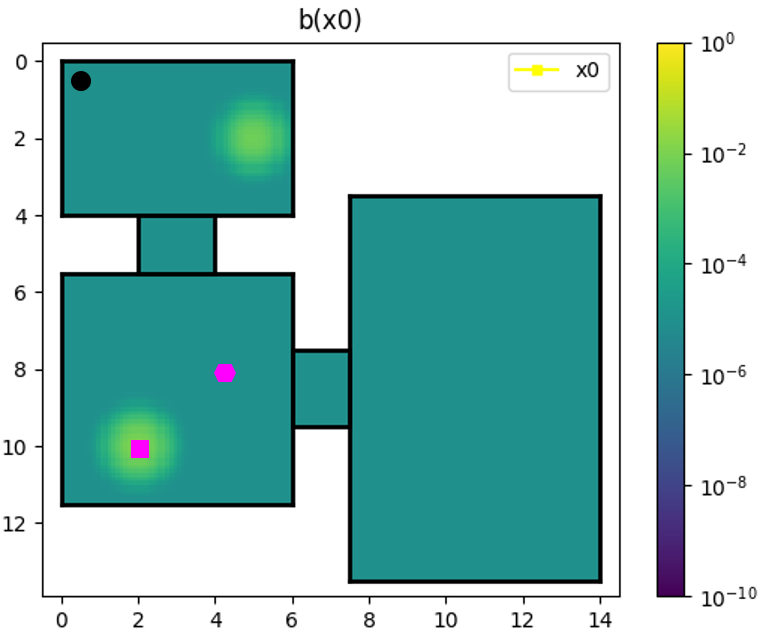
\includegraphics[width=\textwidth]{Report/images/experiments/envsmall_sc01_belief_items.png}
%         \caption{Caption}
%         \label{subfig:my_label}
%     \end{subfigure}
%     \begin{subfigure}[b]{0.49\textwidth}
%          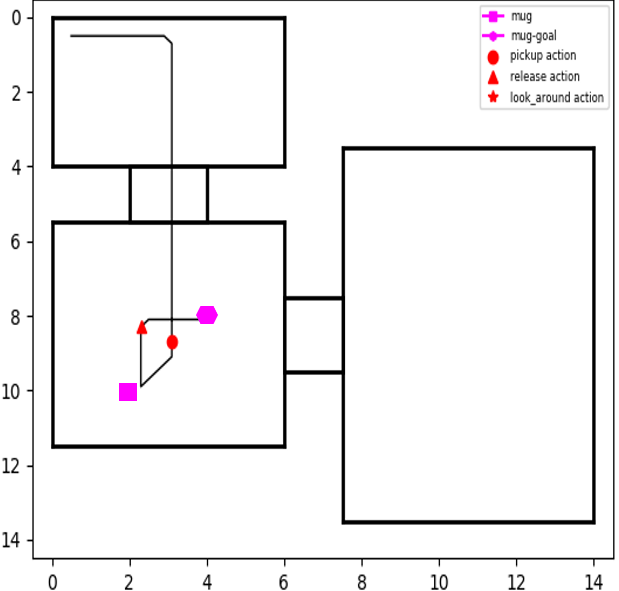
\includegraphics[width=0.82\textwidth]{Report/images/experiments/envsmall_sc01_sol_D1_edited.png}
%         \caption{Caption}
%         \label{subfig:my_label}
%     \end{subfigure}
%     \caption{Blabliblub}
%     \label{fig:my_label}
% \end{figure}

% %%%%%%%%%%%%%%%%%%%%%%%%%%%%%%%%%%%%%%%%%%%%%%%%%%%%%%%%%%%%%%%%%%%%%%%%%%%%%%%%%%%%%
% %%%%%%%%%%%%%%%%%%%%%%%%%%%%%%%%%%%%%%%%%%%%%%%%%%%%%%%%%%%%%%%%%%%%%%%%%%%%%%%%%%%%%
% \begin{figure}
%     \centering
%     \begin{subfigure}[b]{0.49\textwidth}
%         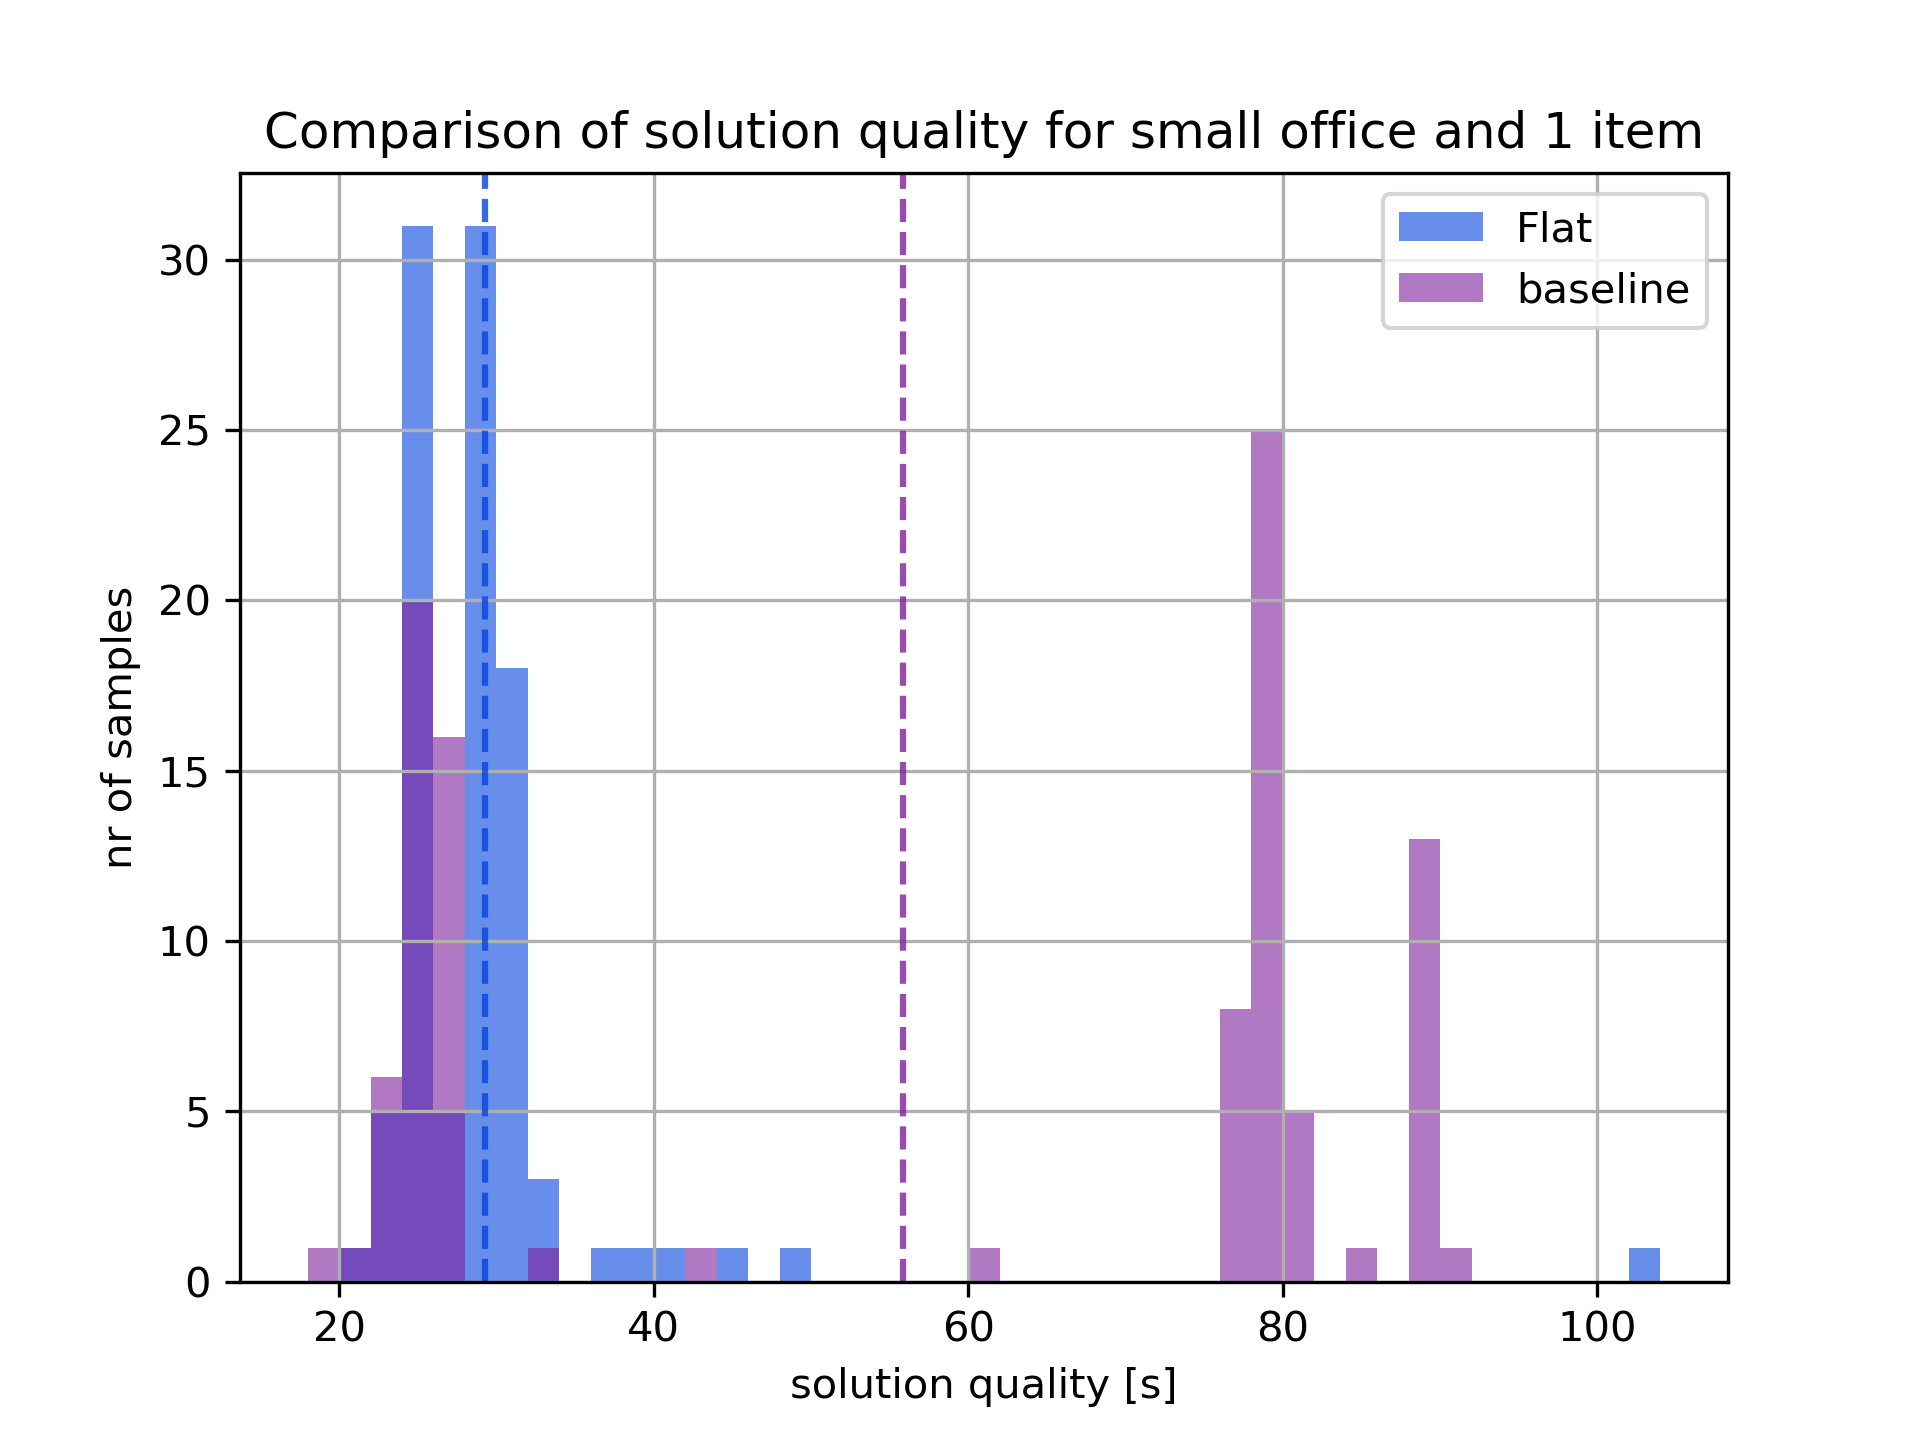
\includegraphics[width=\textwidth]{Report/images/sol_quality/envsmall_sc01_solqual_hist.png}
%         \caption{Caption}
%         \label{subfig:my_label}
%     \end{subfigure}
%     \begin{subfigure}[b]{0.49\textwidth}
%          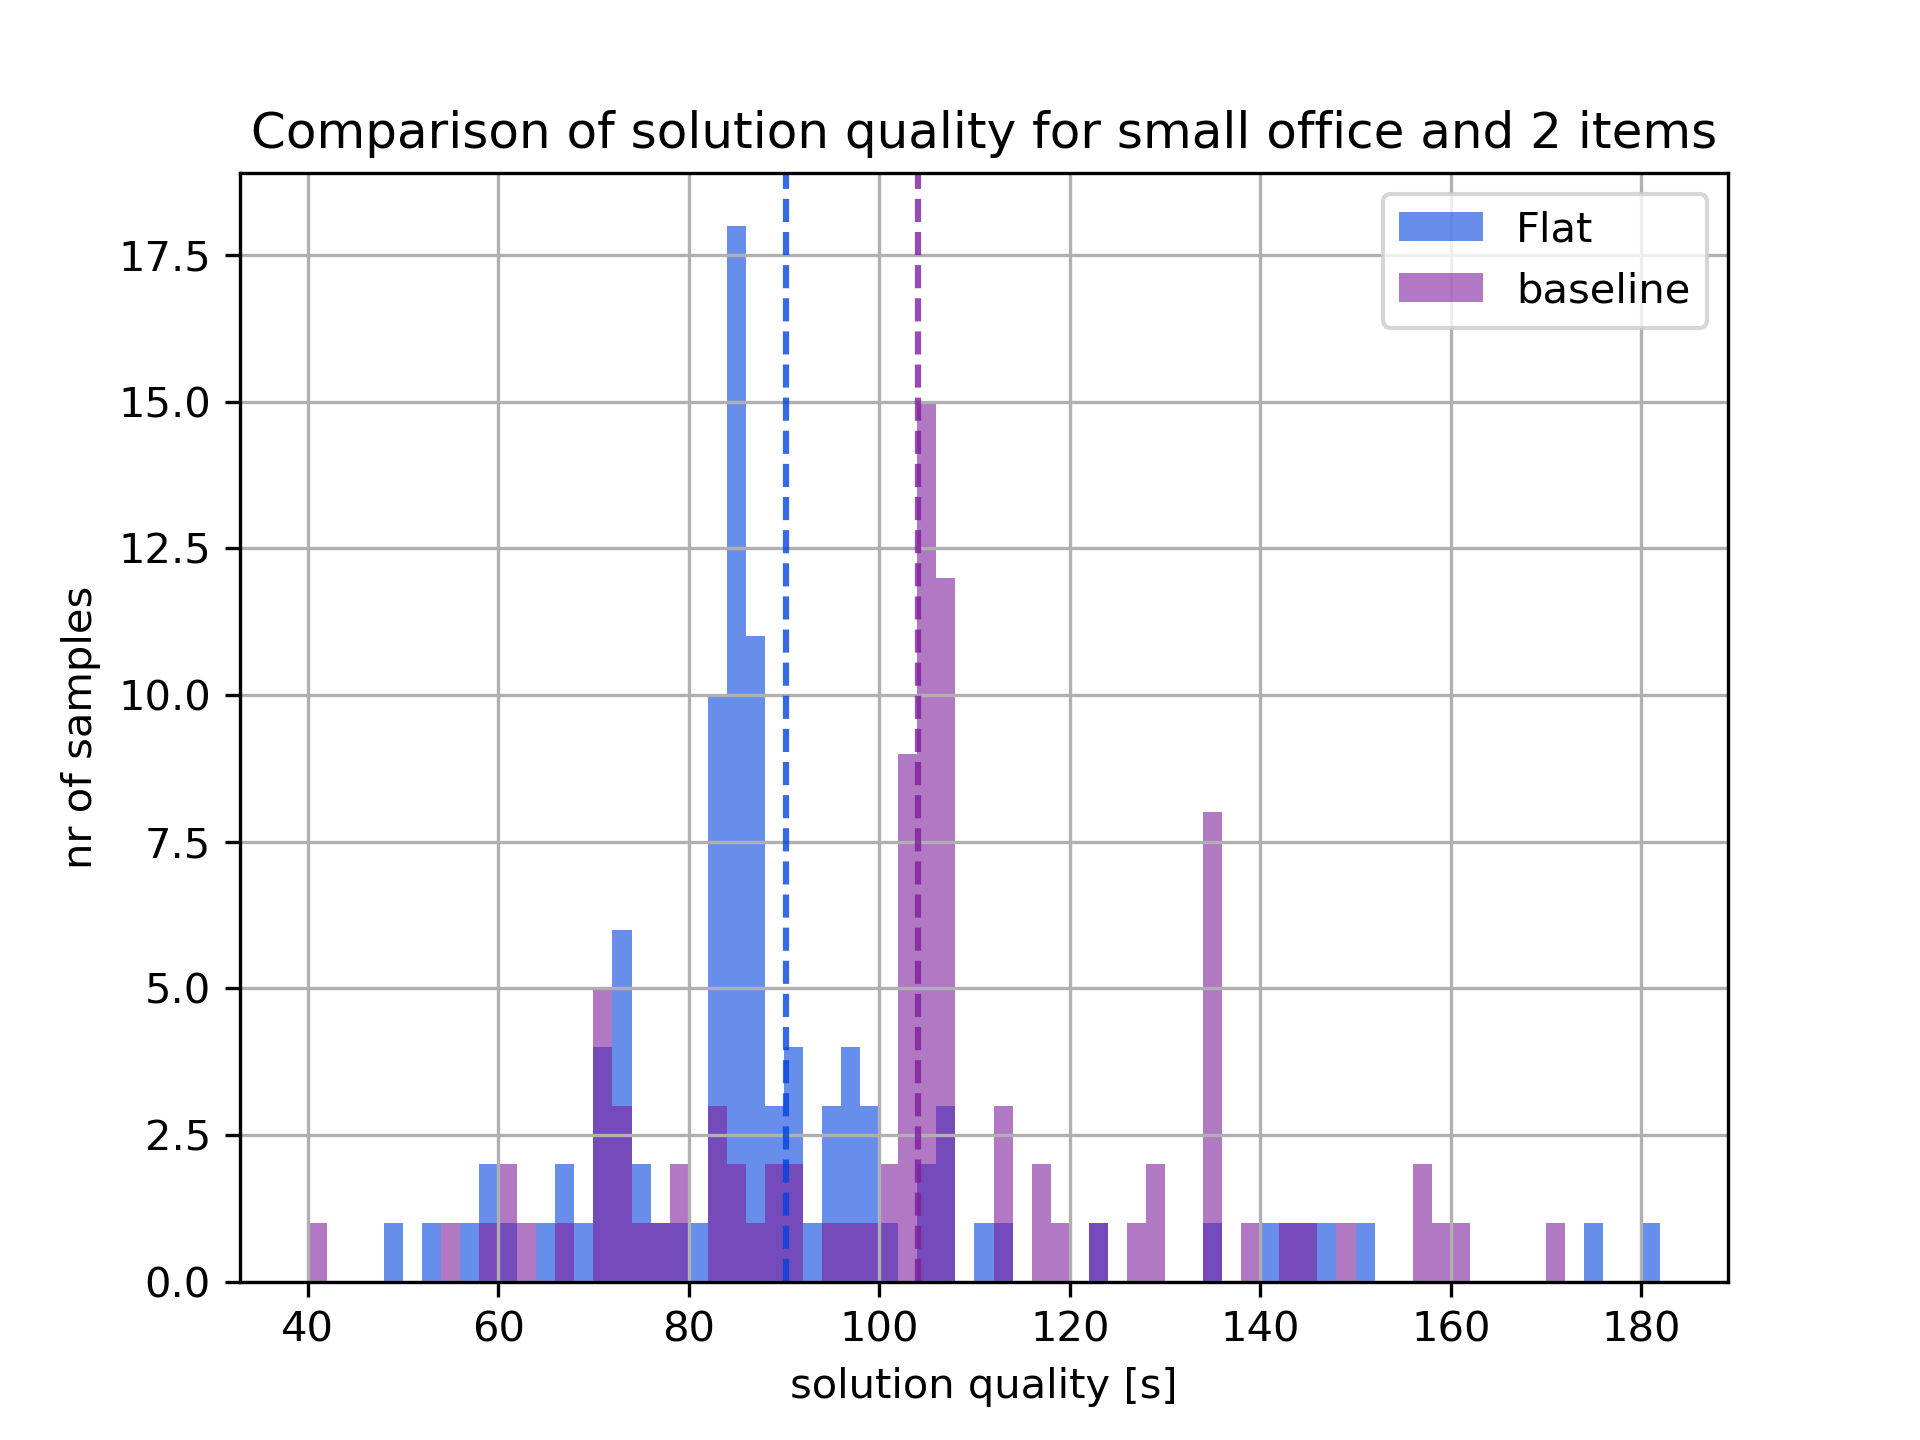
\includegraphics[width=\textwidth]{Report/images/sol_quality/envsmall_sc04_solqual_hist.png}
%         \caption{Caption}
%         \label{subfig:my_label}
%     \end{subfigure}
%     \hfill
%     \begin{subfigure}[b]{0.49\textwidth}
%         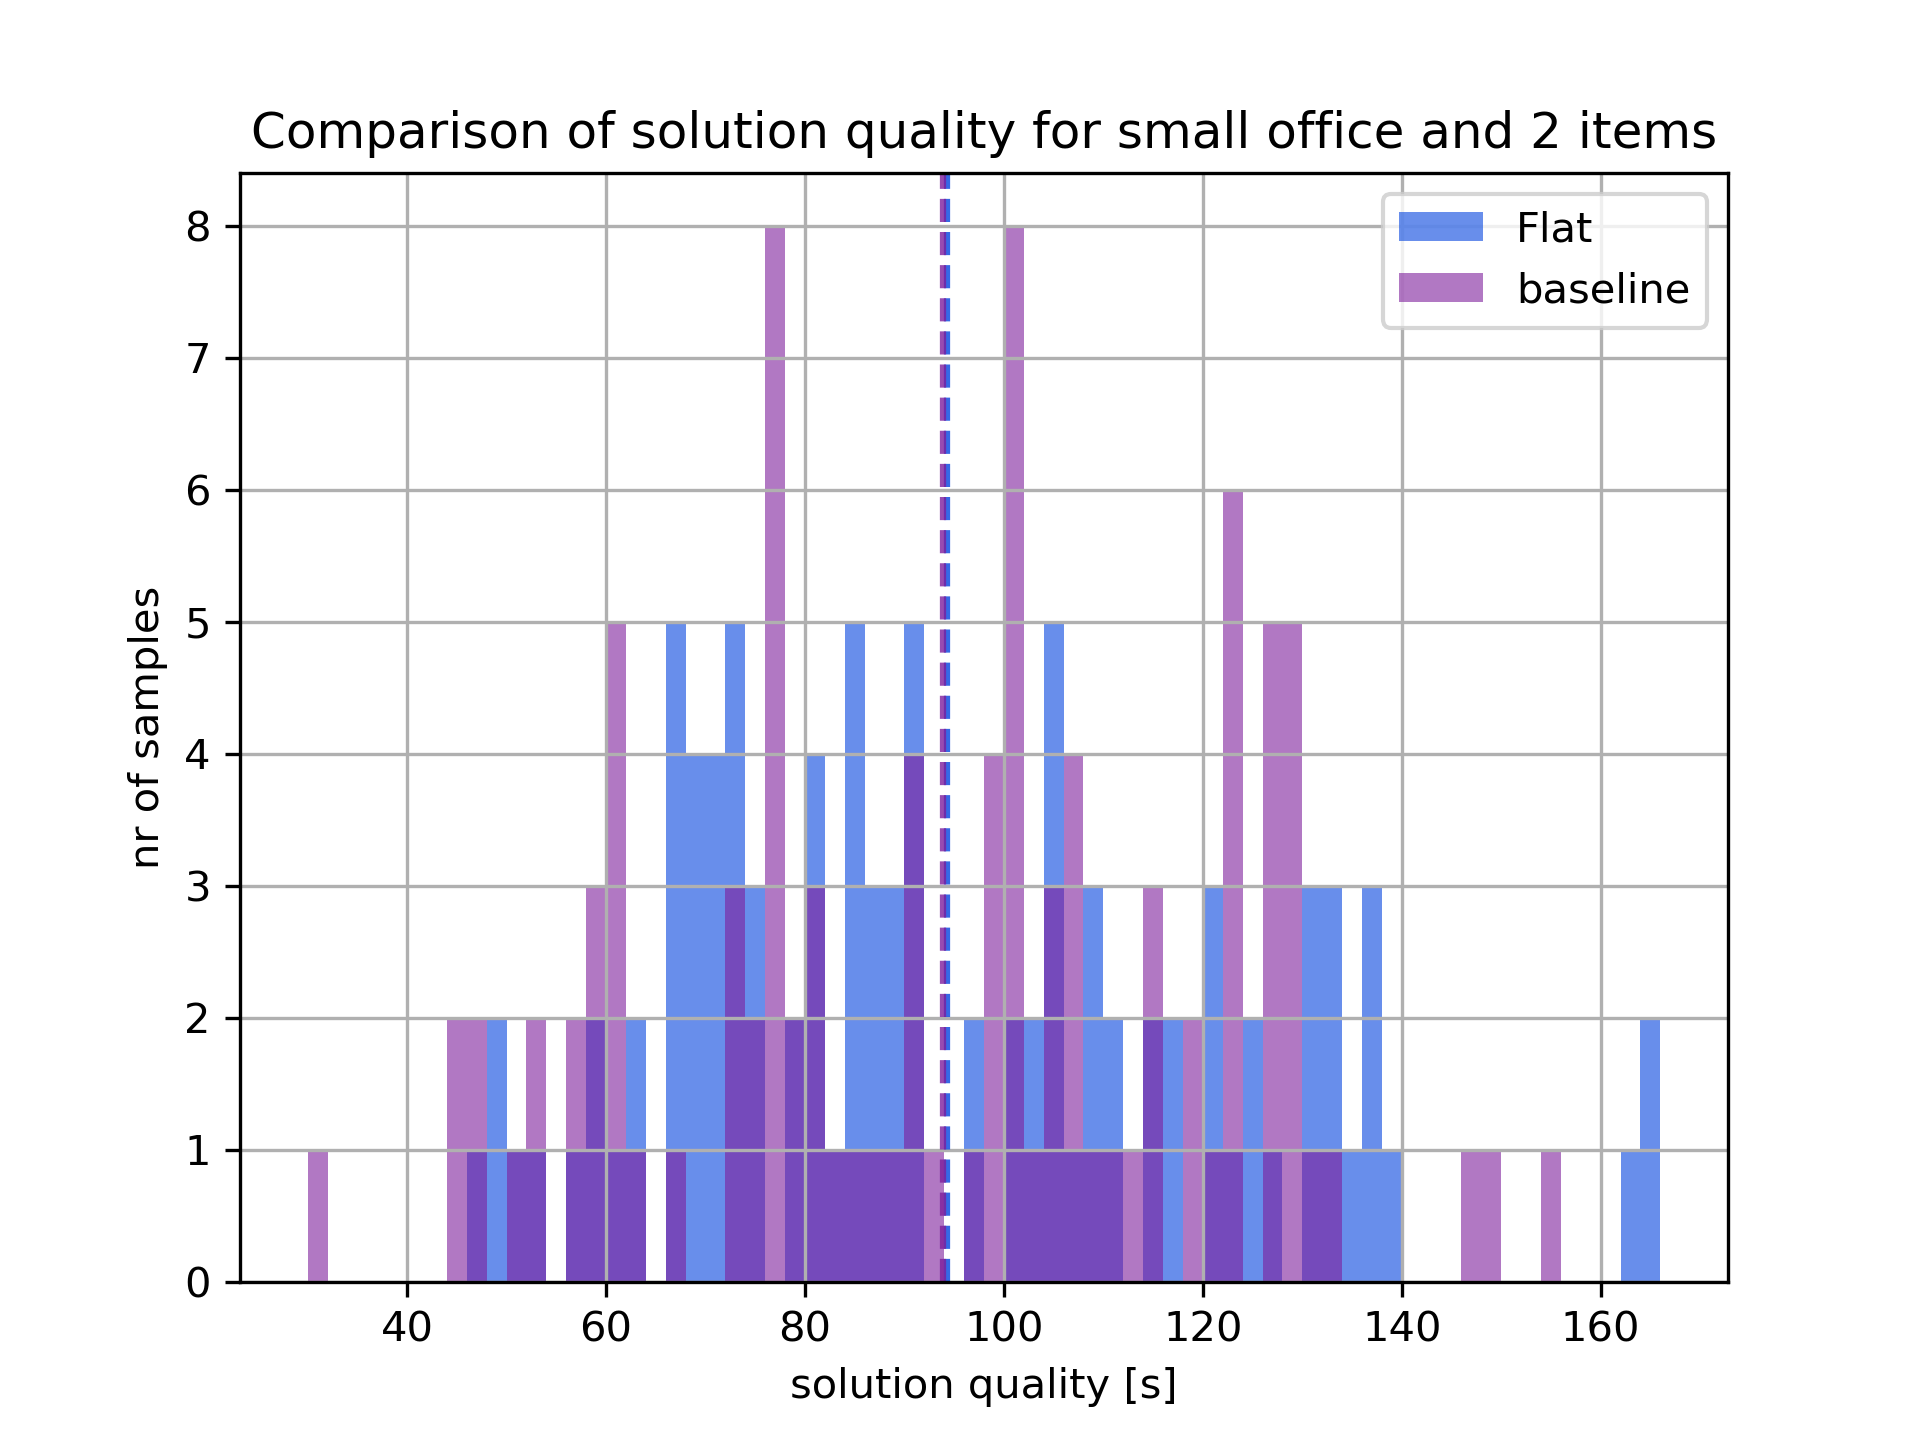
\includegraphics[width=\textwidth]{Report/images/sol_quality/envsmall_sc06_solqual_hist.png}
%         \caption{Caption}
%         \label{subfig:my_label}
%     \end{subfigure}
%     \hfill
%     \begin{subfigure}[b]{0.49\textwidth}
%          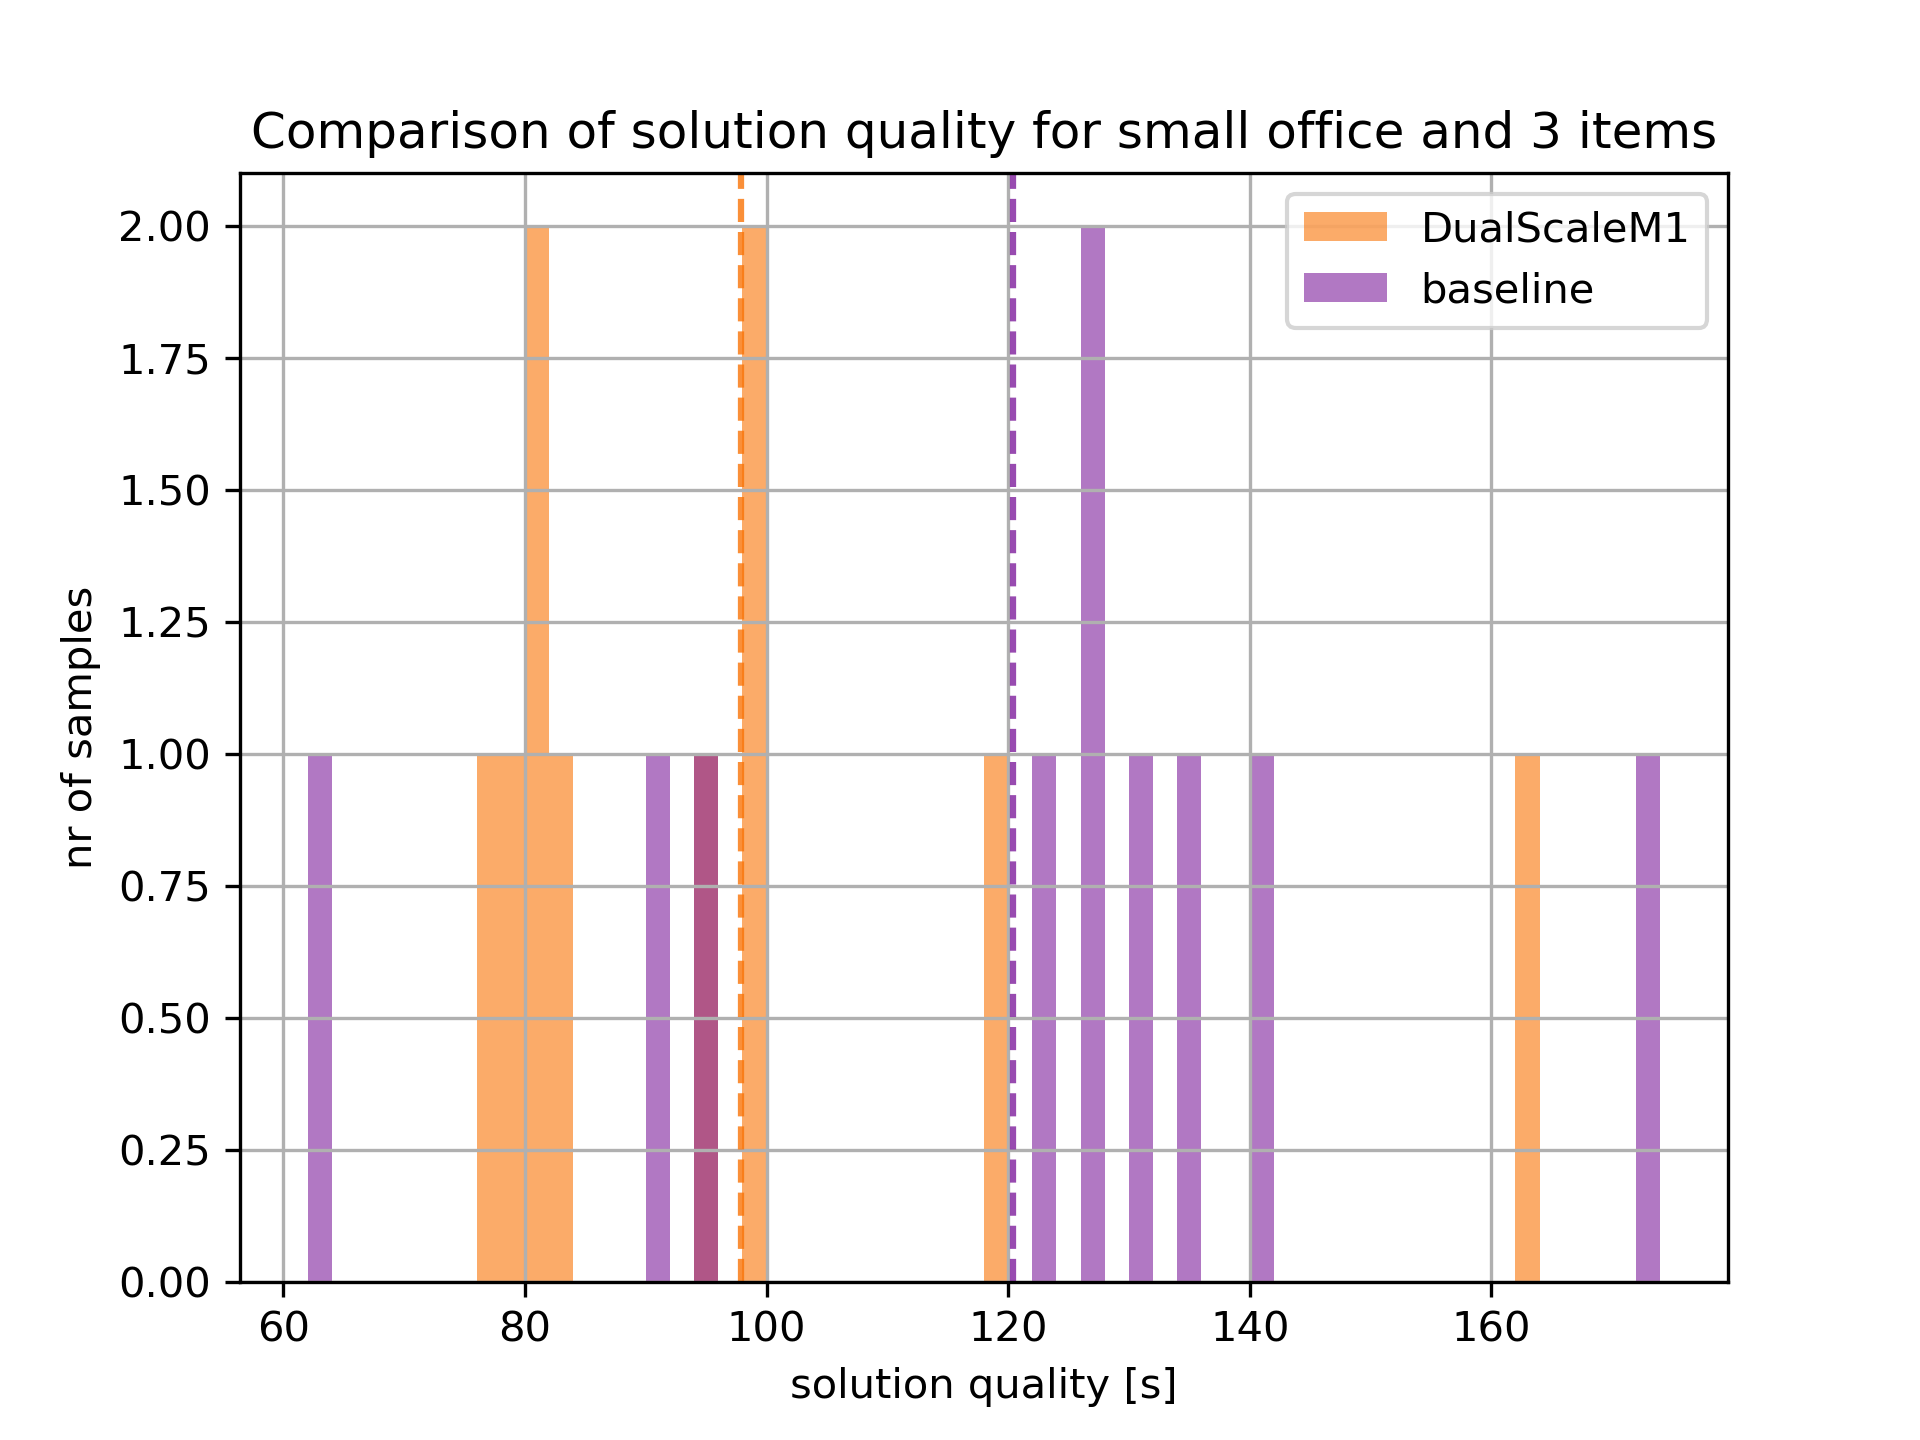
\includegraphics[width=\textwidth]{Report/images/sol_quality/envsmall_sc09_solqual_hist.png}
%         \caption{Caption}
%         \label{subfig:my_label}
%     \end{subfigure}
%     \caption{Blabliblub}
%     \label{fig:my_label}
% \end{figure}
% %%%%%%%%%%%%%%%%%%%%%%%%%%%%%%%%%%%%%%%%%%%%%%%%%%%%%%%%%%%%%%%%%%%%%%%%%%%%%%%%%
% %%%%%%%%%%%%%%%%%%%%%%%%%%%%%%%%%%%%%%%%%%%%%%%%%%%%%%%%%%%%%%%%%%%%%%%%%%%%%%%%%
% \begin{figure}
%     \centering
%     \begin{subfigure}[b]{0.49\textwidth}
%         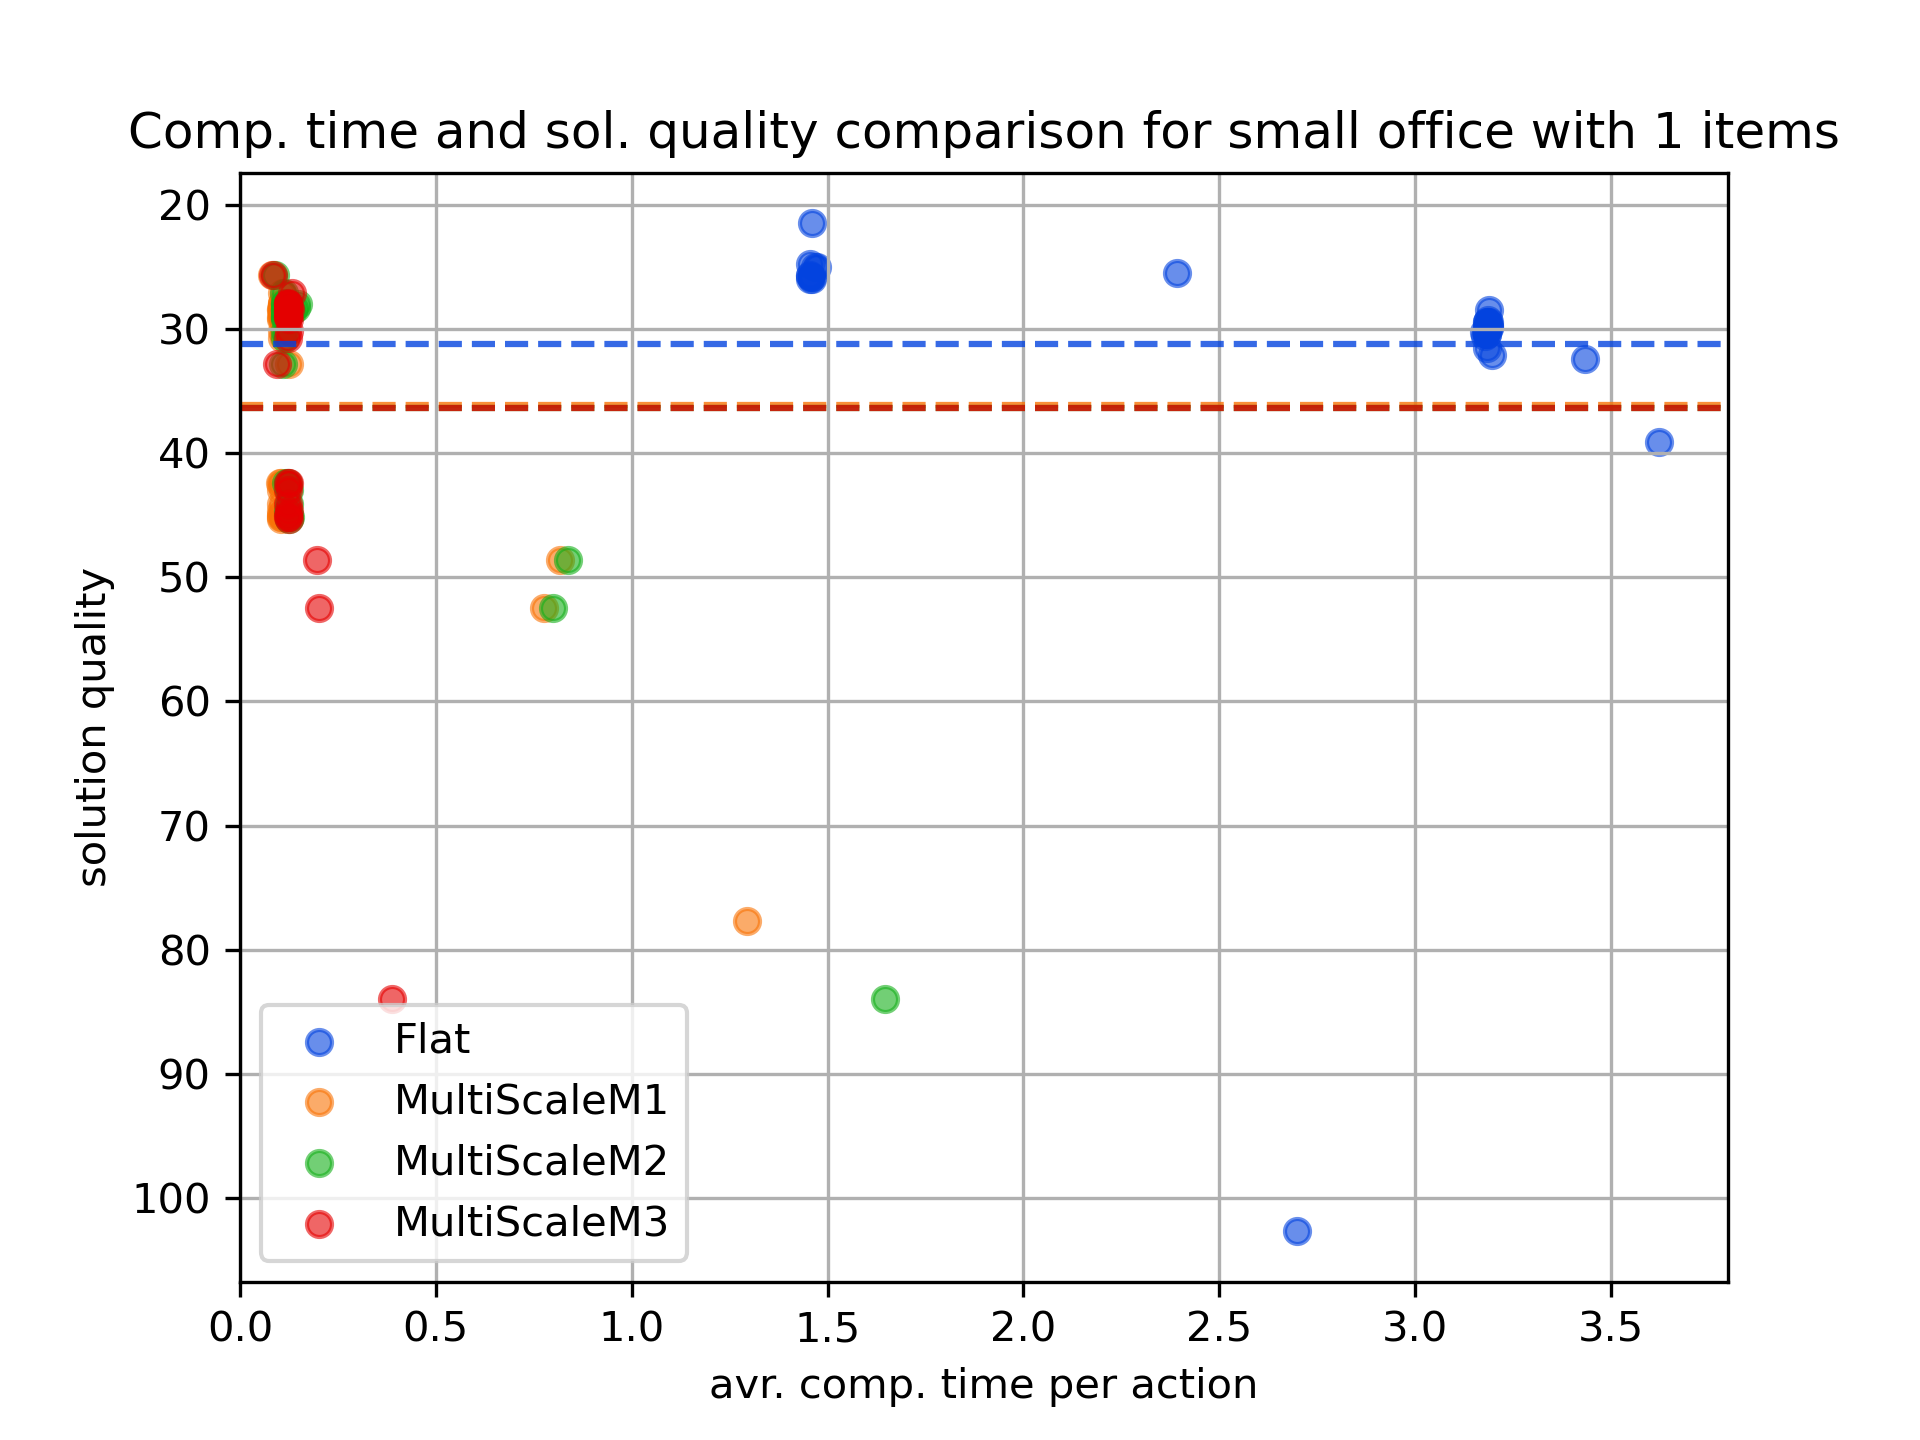
\includegraphics[width=\textwidth]{Report/images/comp_time_vs_sol_quality/envsmall_sc01_scatter_comptimes_vs_solqual.png}
%         \caption{Caption}
%         \label{subfig:my_label}
%     \end{subfigure}
%     \begin{subfigure}[b]{0.49\textwidth}
%          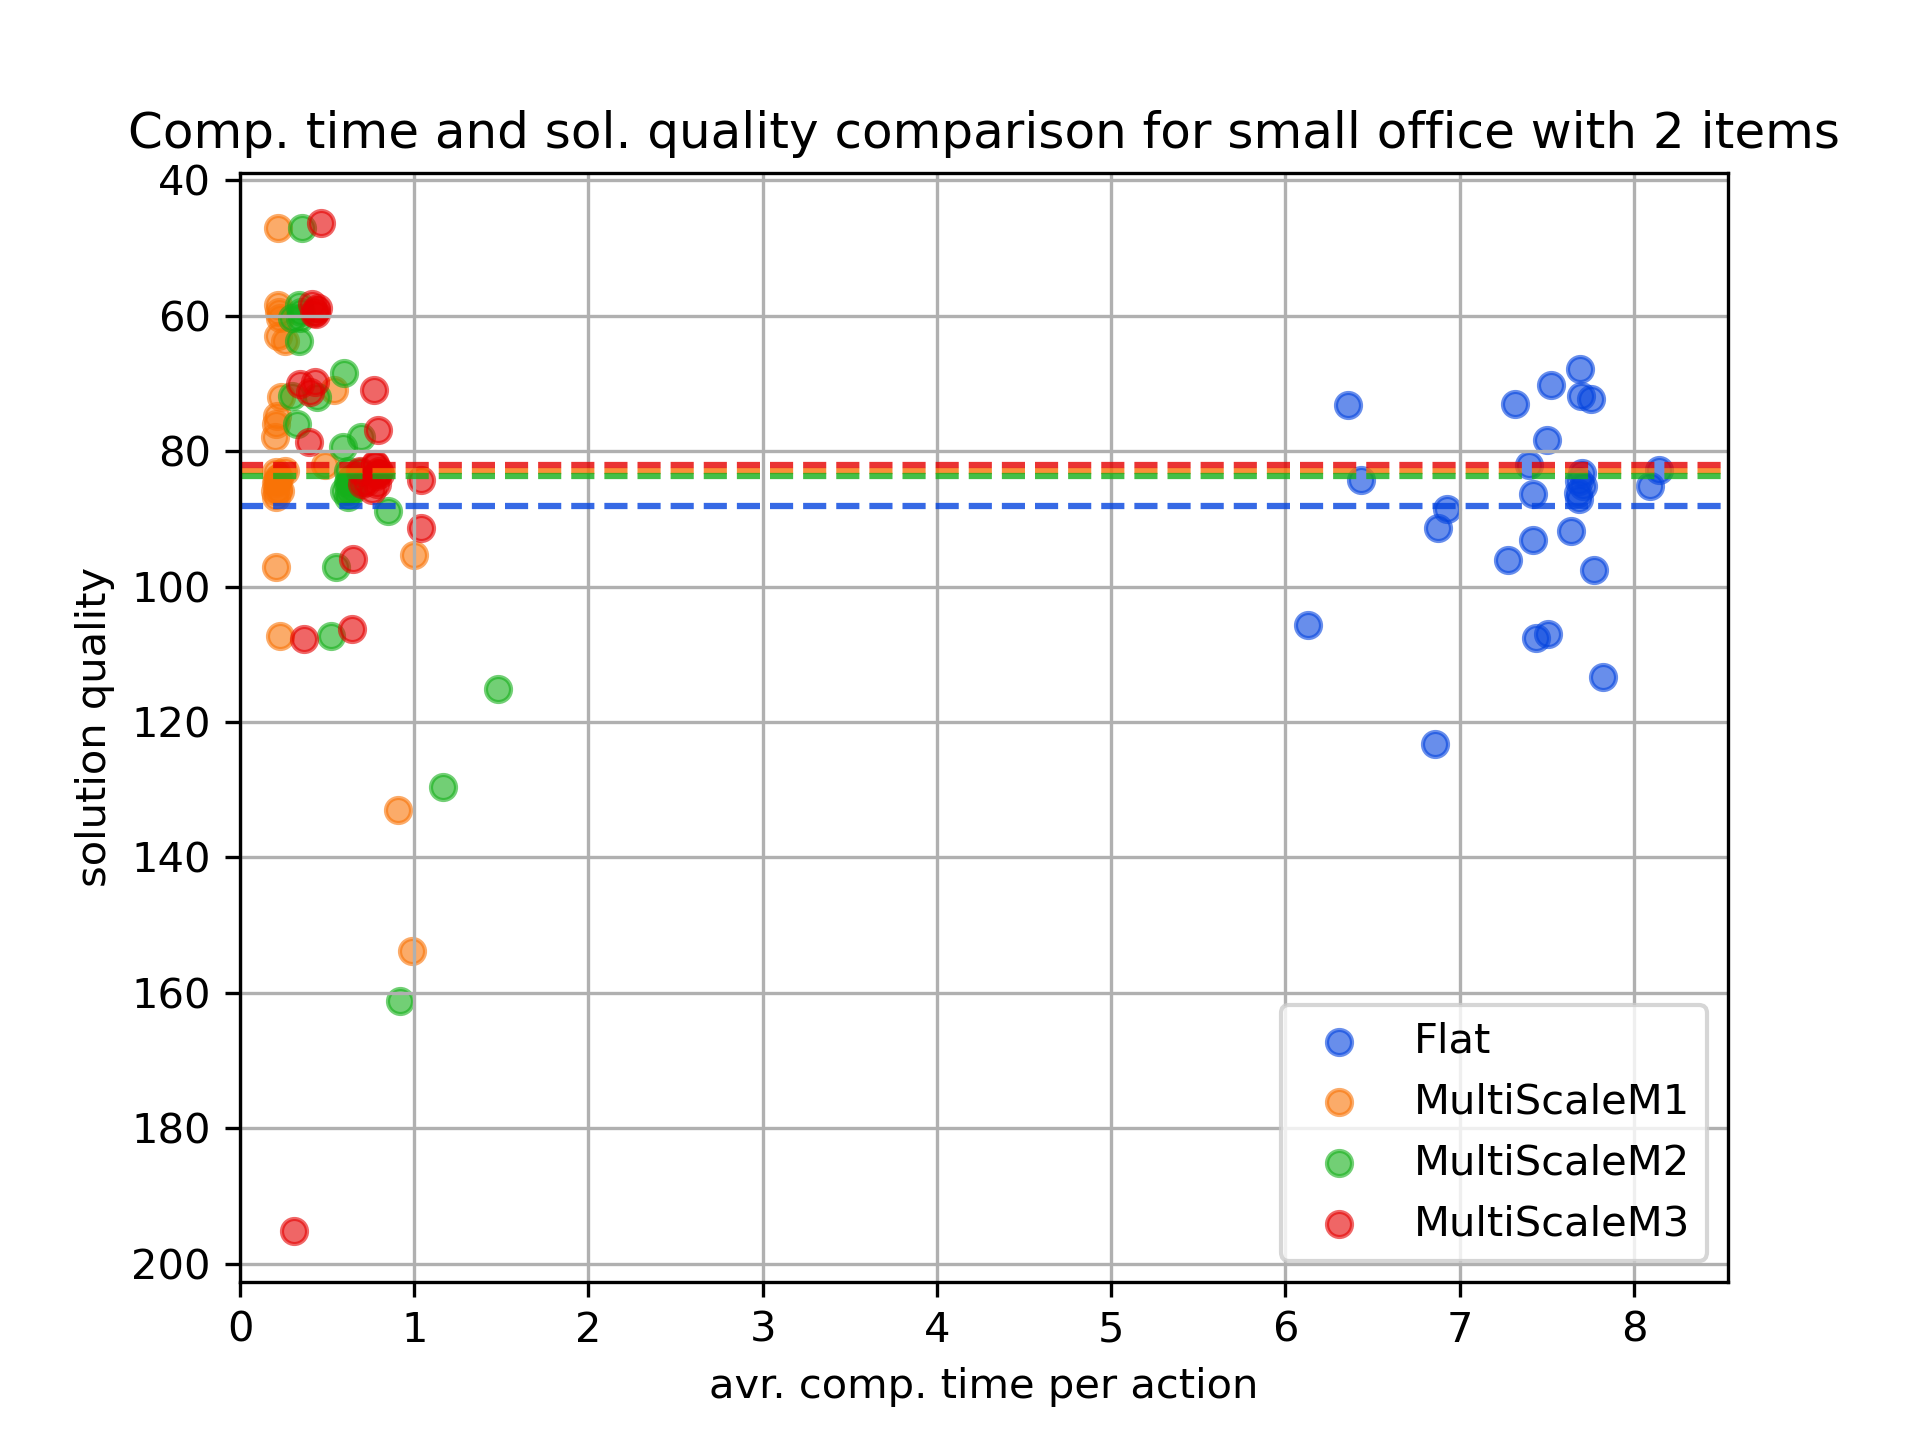
\includegraphics[width=\textwidth]{Report/images/comp_time_vs_sol_quality/envsmall_sc04_scatter_comptimes_vs_solqual.png}
%         \caption{Caption}
%         \label{subfig:my_label}
%     \end{subfigure}
%     \hfill
%     \begin{subfigure}[b]{0.49\textwidth}
%         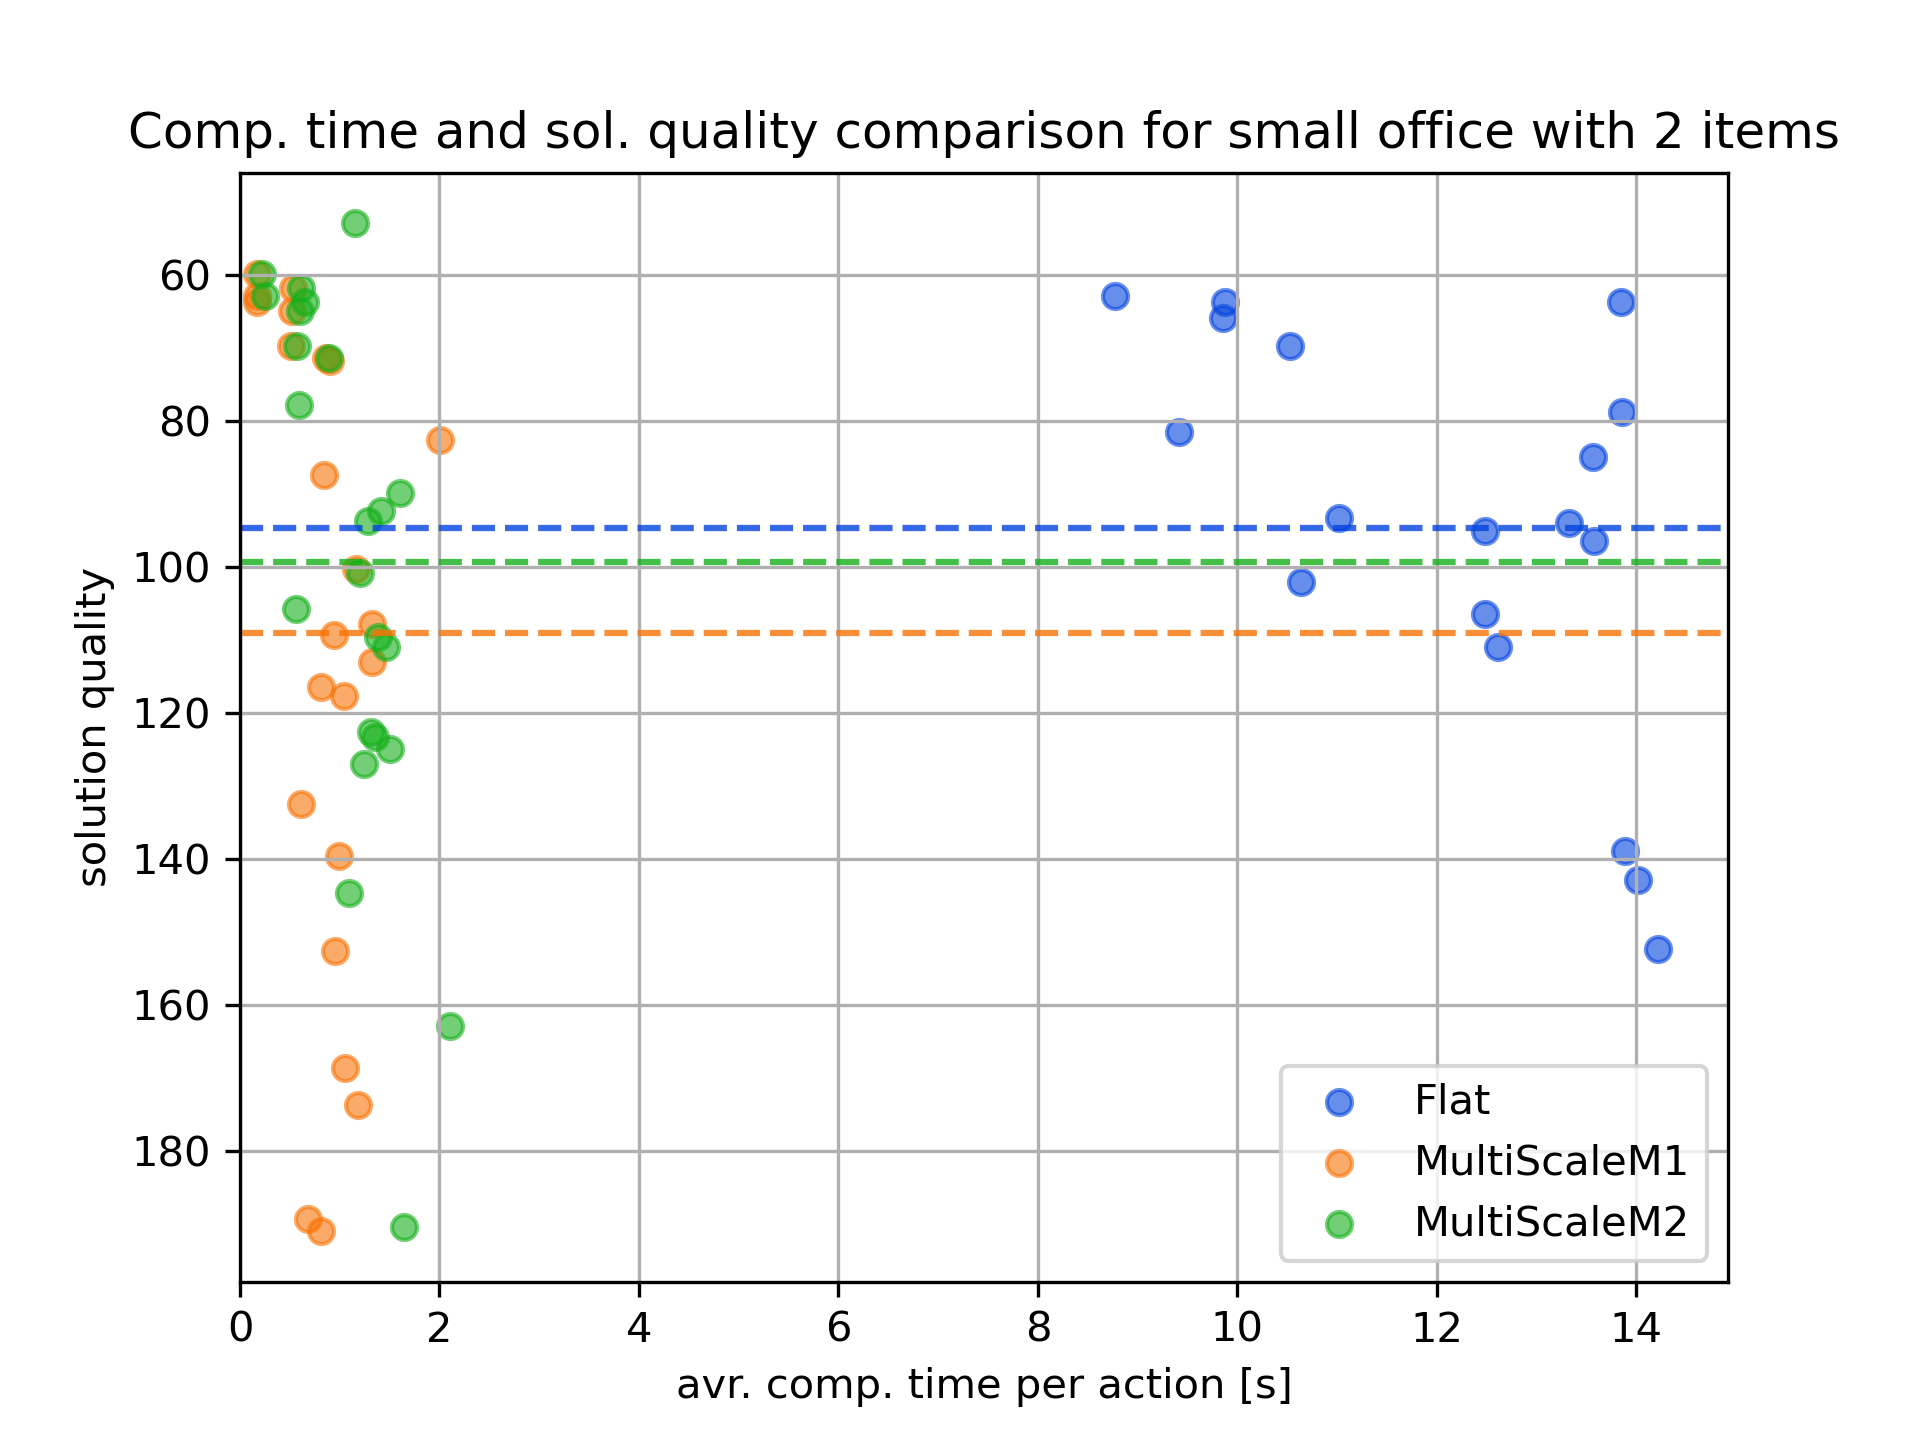
\includegraphics[width=\textwidth]{Report/images/comp_time_vs_sol_quality/envsmall_sc08_scatter_comptimes_vs_solqual.png}
%         \caption{Caption}
%         \label{subfig:my_label}
%     \end{subfigure}
%     \hfill
%     \begin{subfigure}[b]{0.49\textwidth}
%          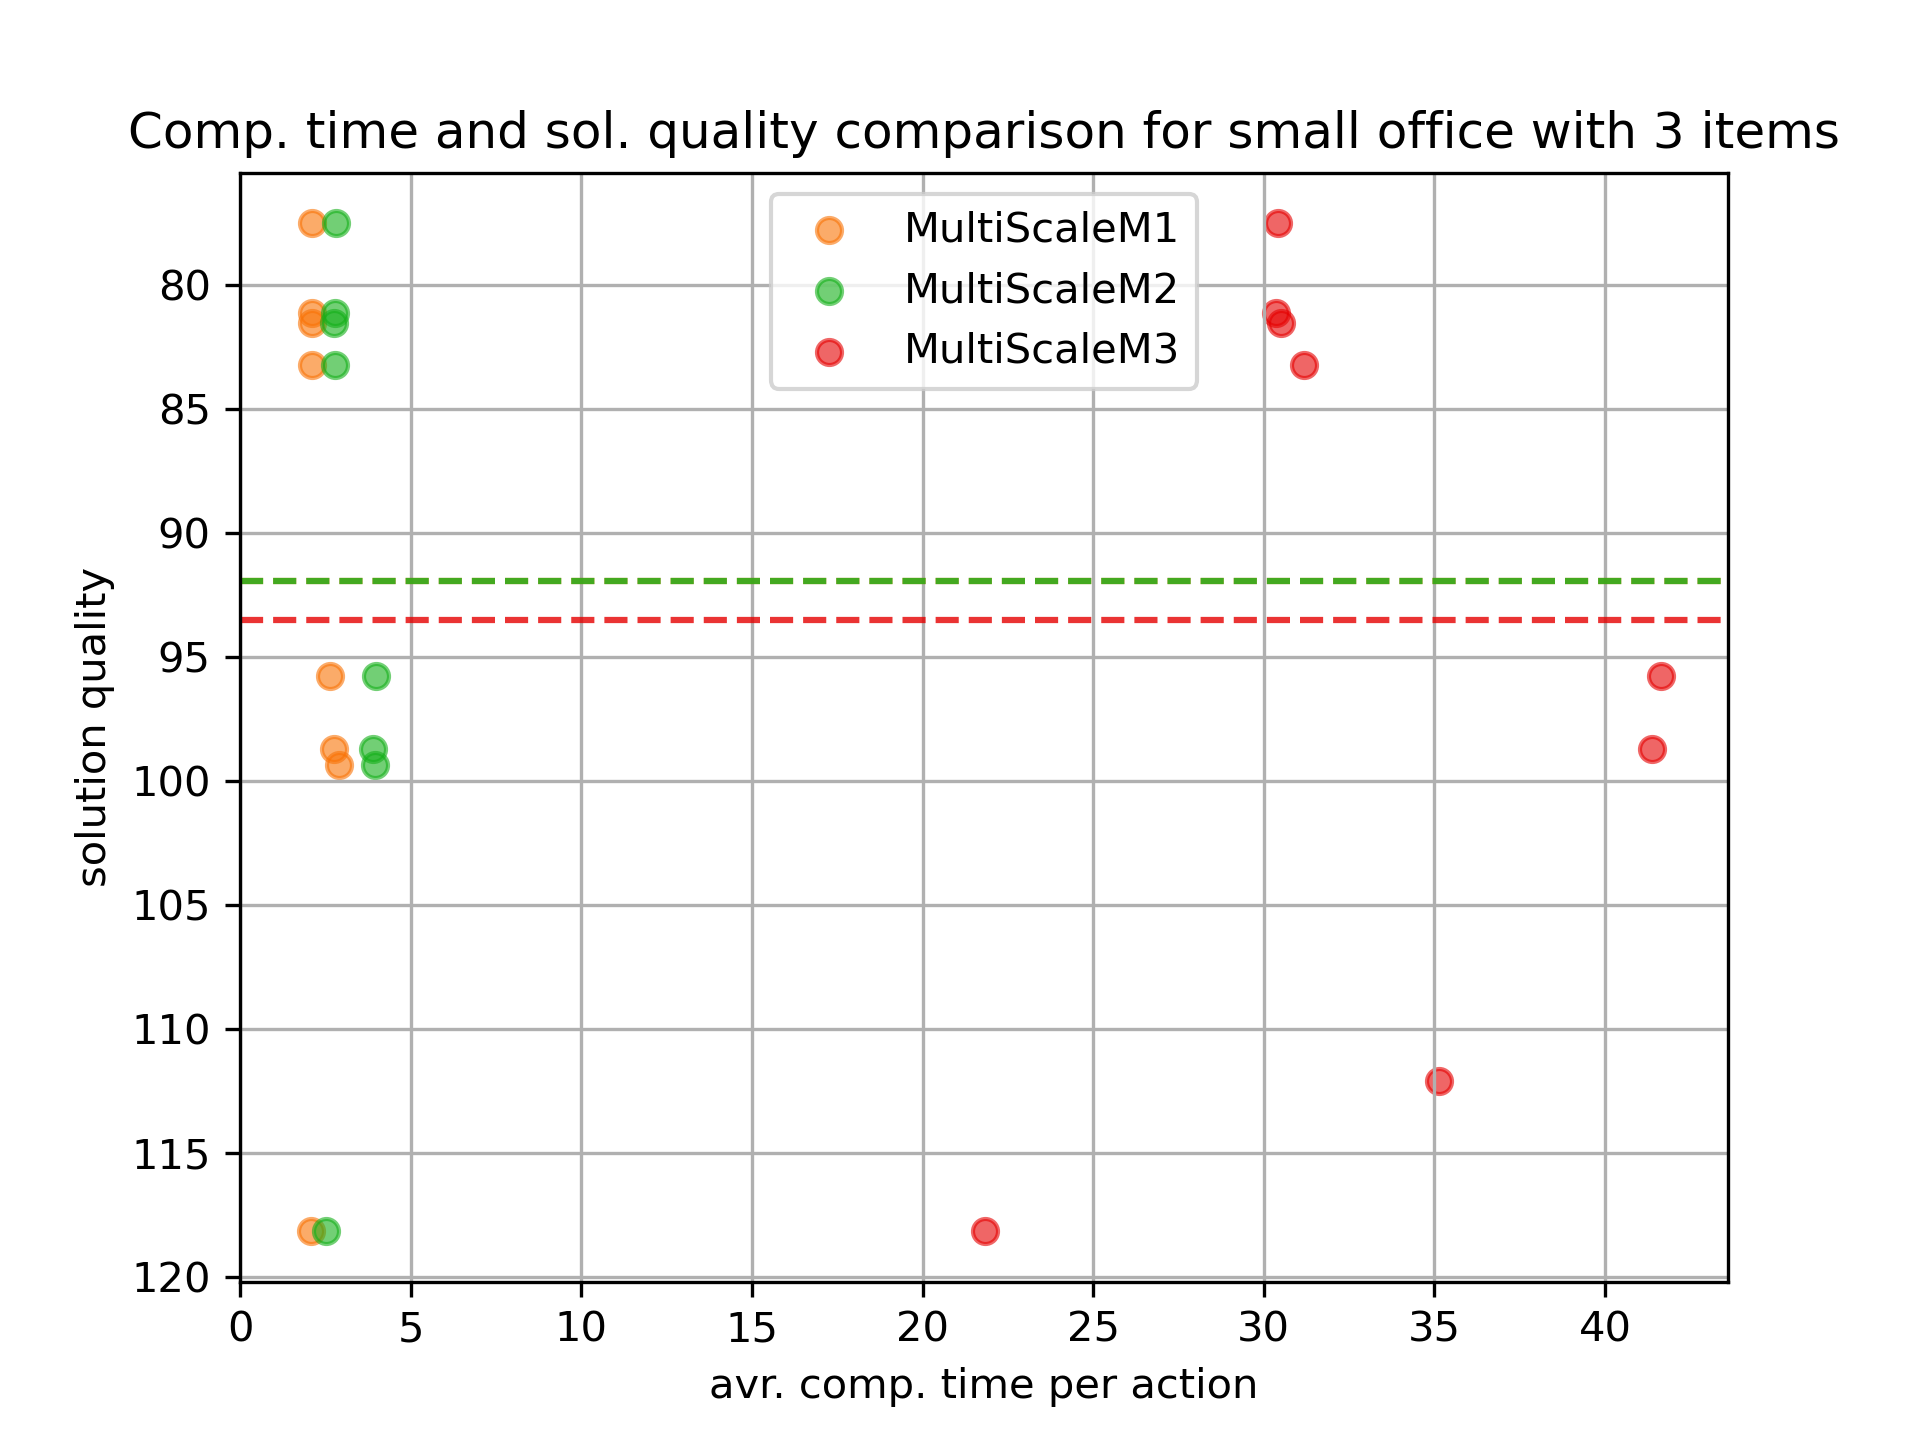
\includegraphics[width=\textwidth]{Report/images/comp_time_vs_sol_quality/envsmall_sc09_scatter_comptimes_vs_solqual.png}
%         \caption{Caption}
%         \label{subfig:my_label}
%     \end{subfigure}
%         \hfill
%     \begin{subfigure}[b]{0.49\textwidth}
%         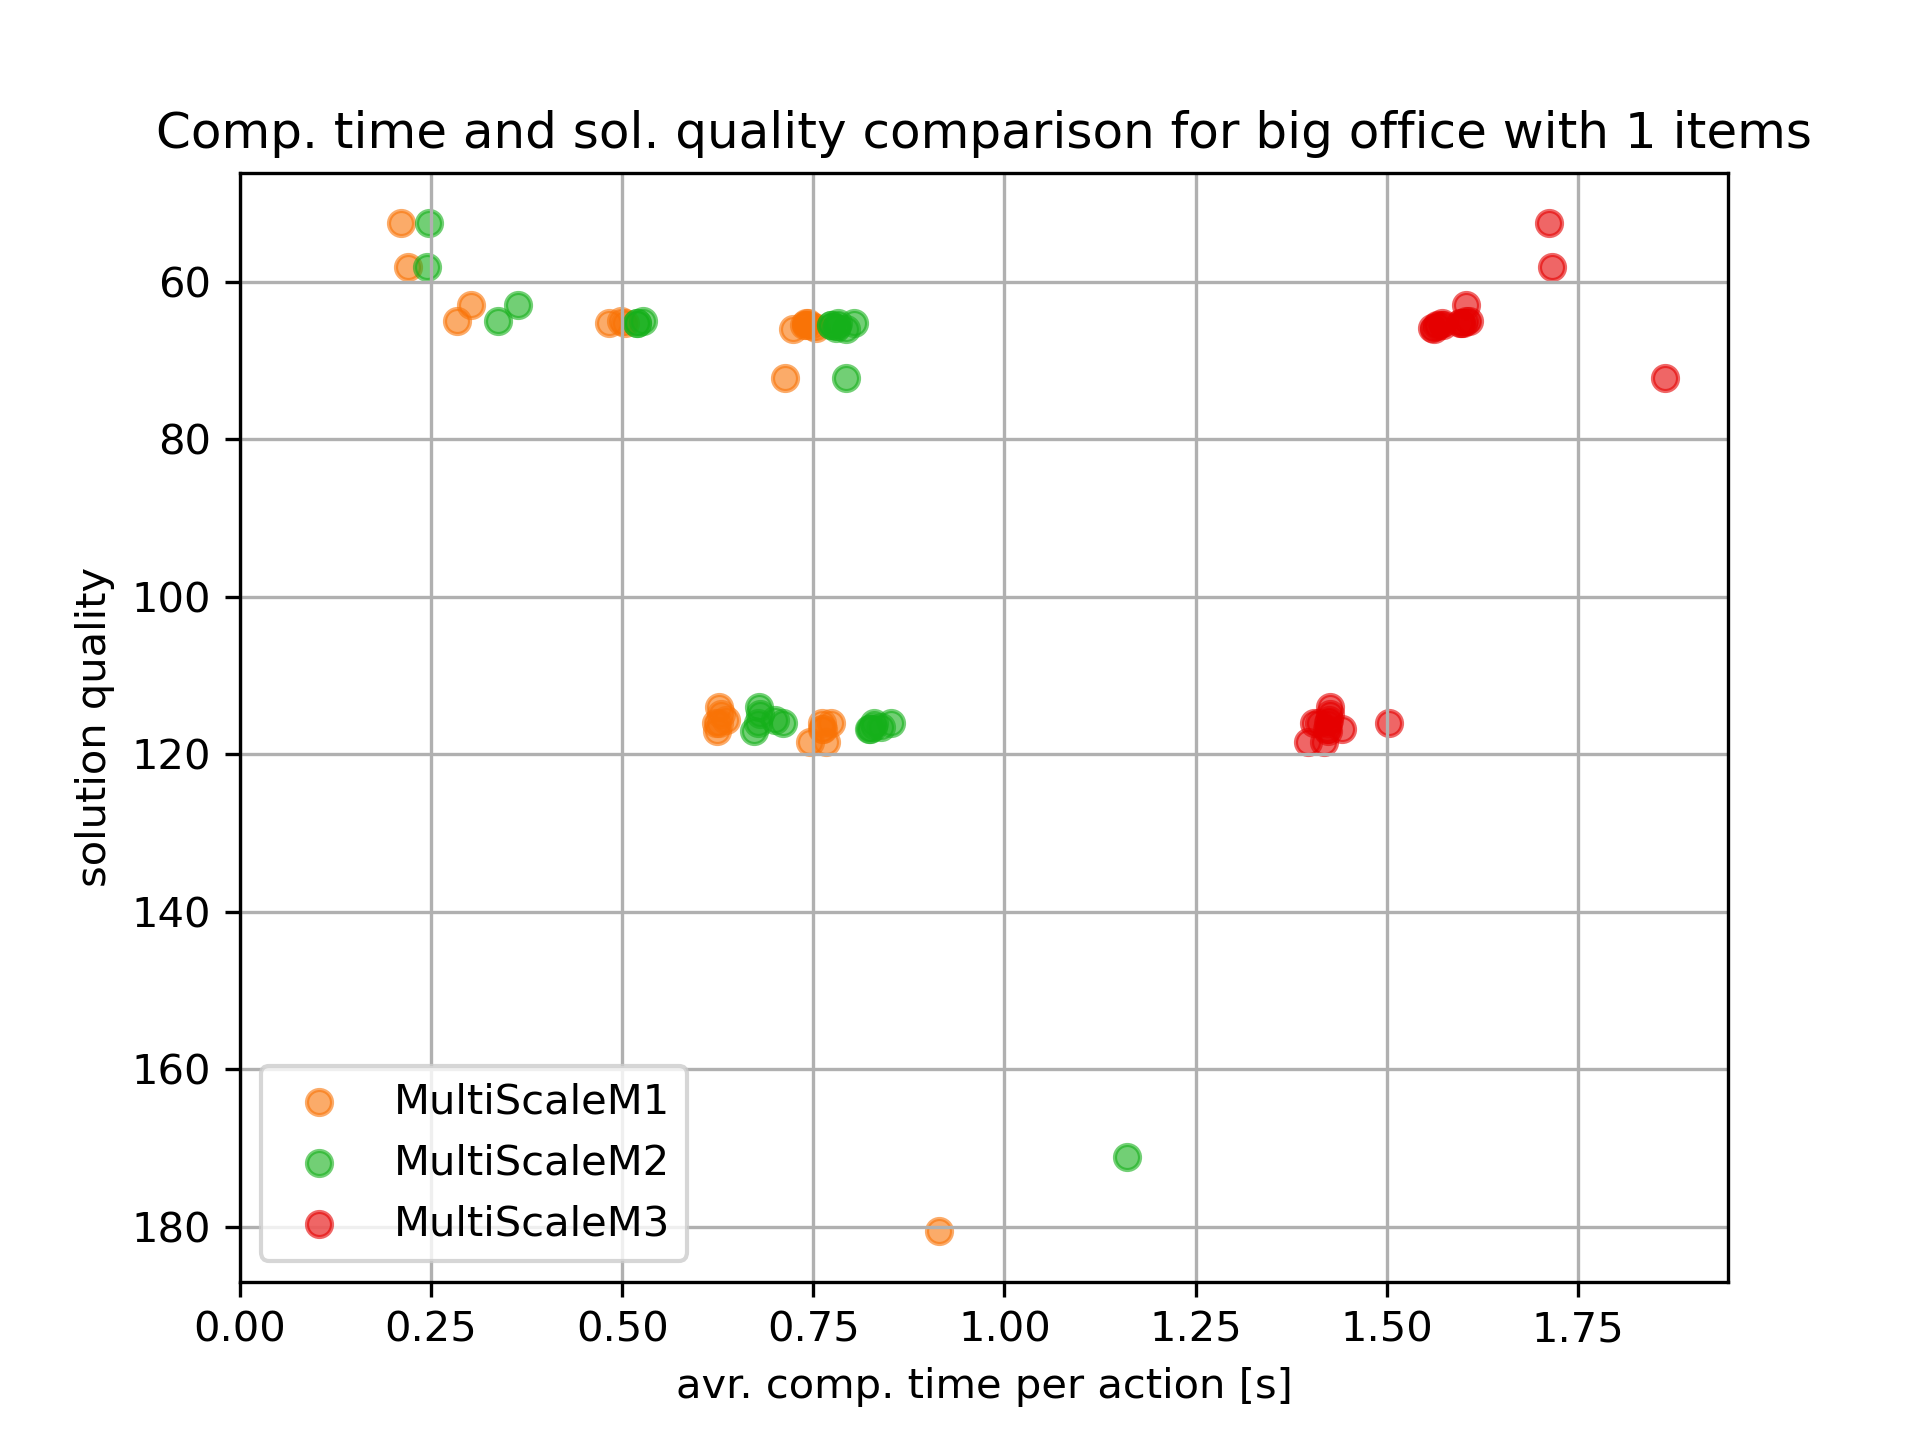
\includegraphics[width=\textwidth]{Report/images/comp_time_vs_sol_quality/envbig_sc01_noavr_scatter_comptimes_vs_solqual.png}
%         \caption{Caption}
%         \label{subfig:my_label}
%     \end{subfigure}
%     \hfill
%     \begin{subfigure}[b]{0.49\textwidth}
%          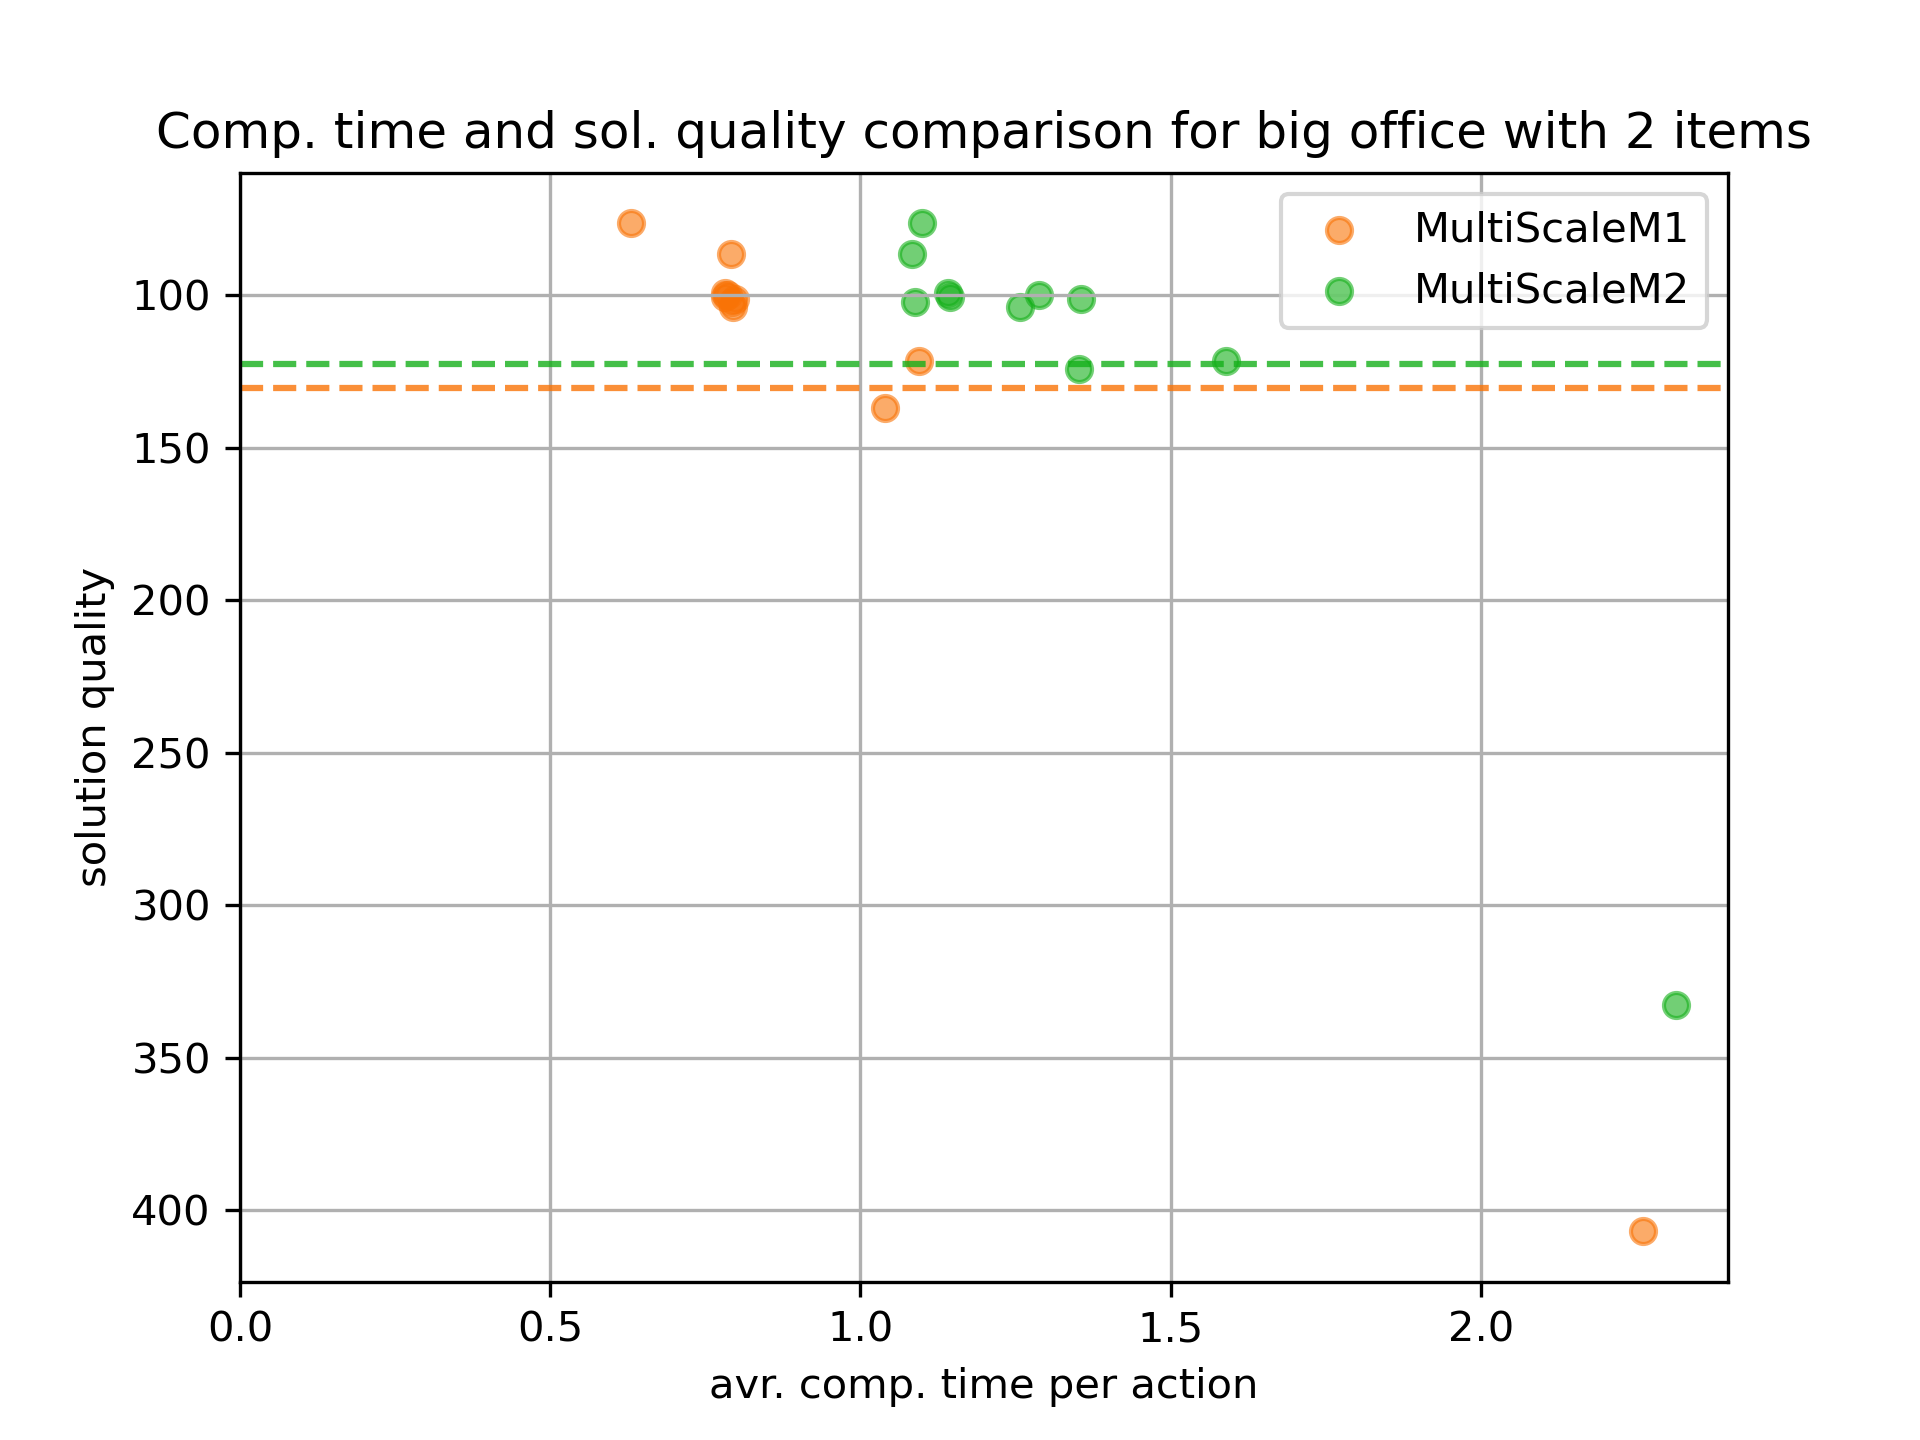
\includegraphics[width=\textwidth]{Report/images/comp_time_vs_sol_quality/envbig_sc03_scatter_comptimes_vs_solqual.png}
%         \caption{Caption}
%         \label{subfig:my_label}
%     \end{subfigure}
%     \caption{Blabliblub}
%     \label{fig:my_label}
% \end{figure}



% %%%%%%%%%%%%%%%%%%%%%%%%%%%%%%%%%%%%%%%%%%%%%%%%%%%%%%%%%%%%%%%%%%%%%%%%%%%%%%%%%
% %%%%%%%%%%%%%%%%%%%%%%%%%%%%%%%%%%%%%%%%%%%%%%%%%%%%%%%%%%%%%%%%%%%%%%%%%%%%%%%%%
% \begin{figure}
%     \centering
%     \begin{subfigure}[b]{0.49\textwidth}
%         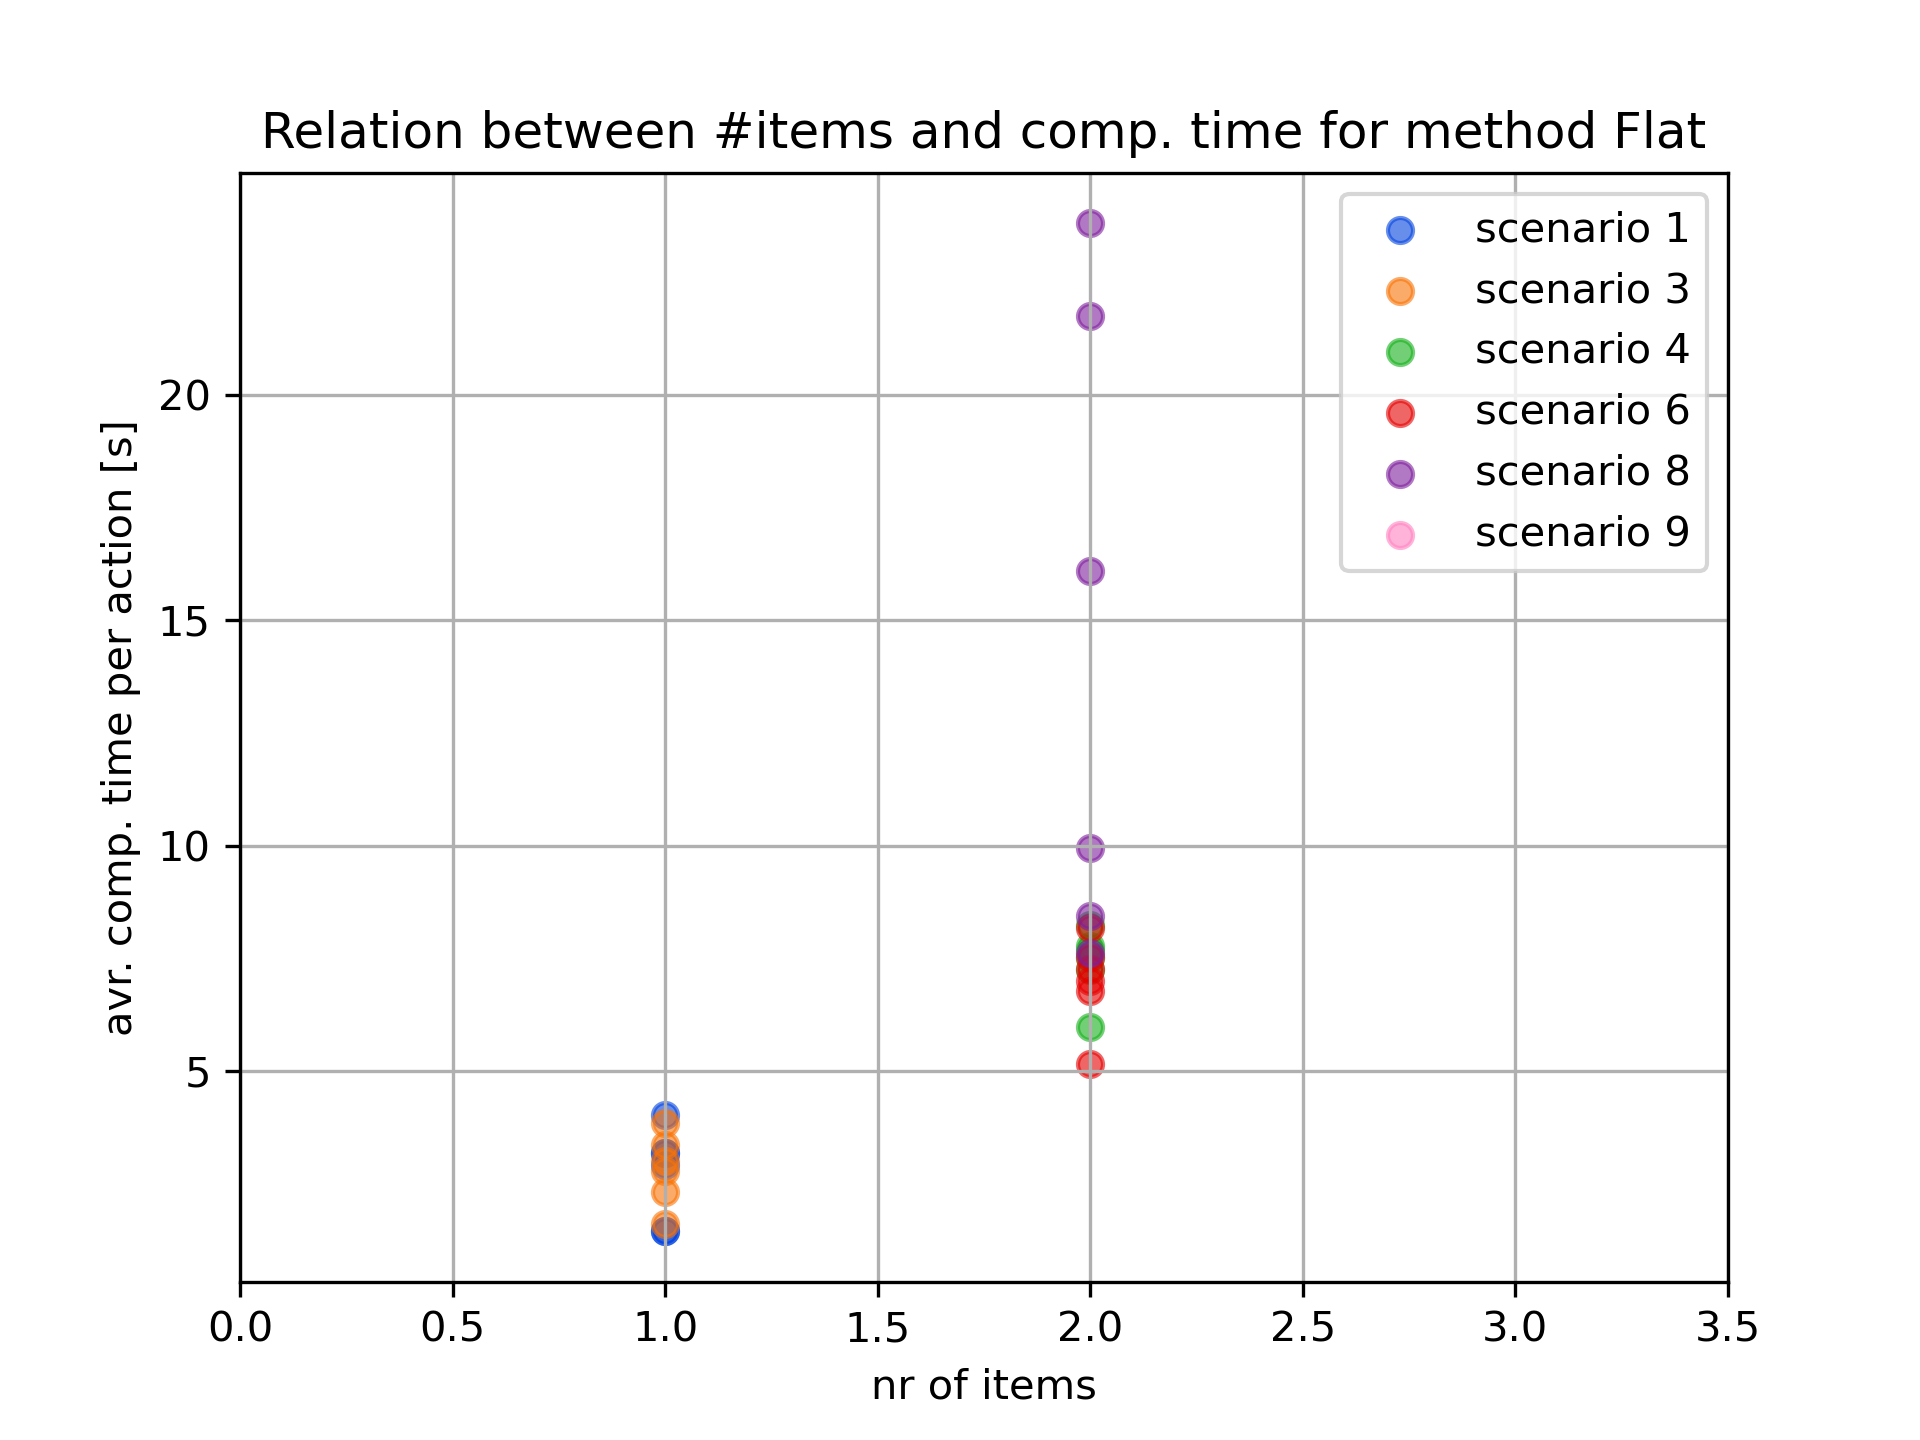
\includegraphics[width=\textwidth]{Report/images/nr_of_items/items_vs_comptime_Flat.png}
%         \caption{Caption}
%         \label{subfig:my_label}
%     \end{subfigure}
%     \begin{subfigure}[b]{0.49\textwidth}
%          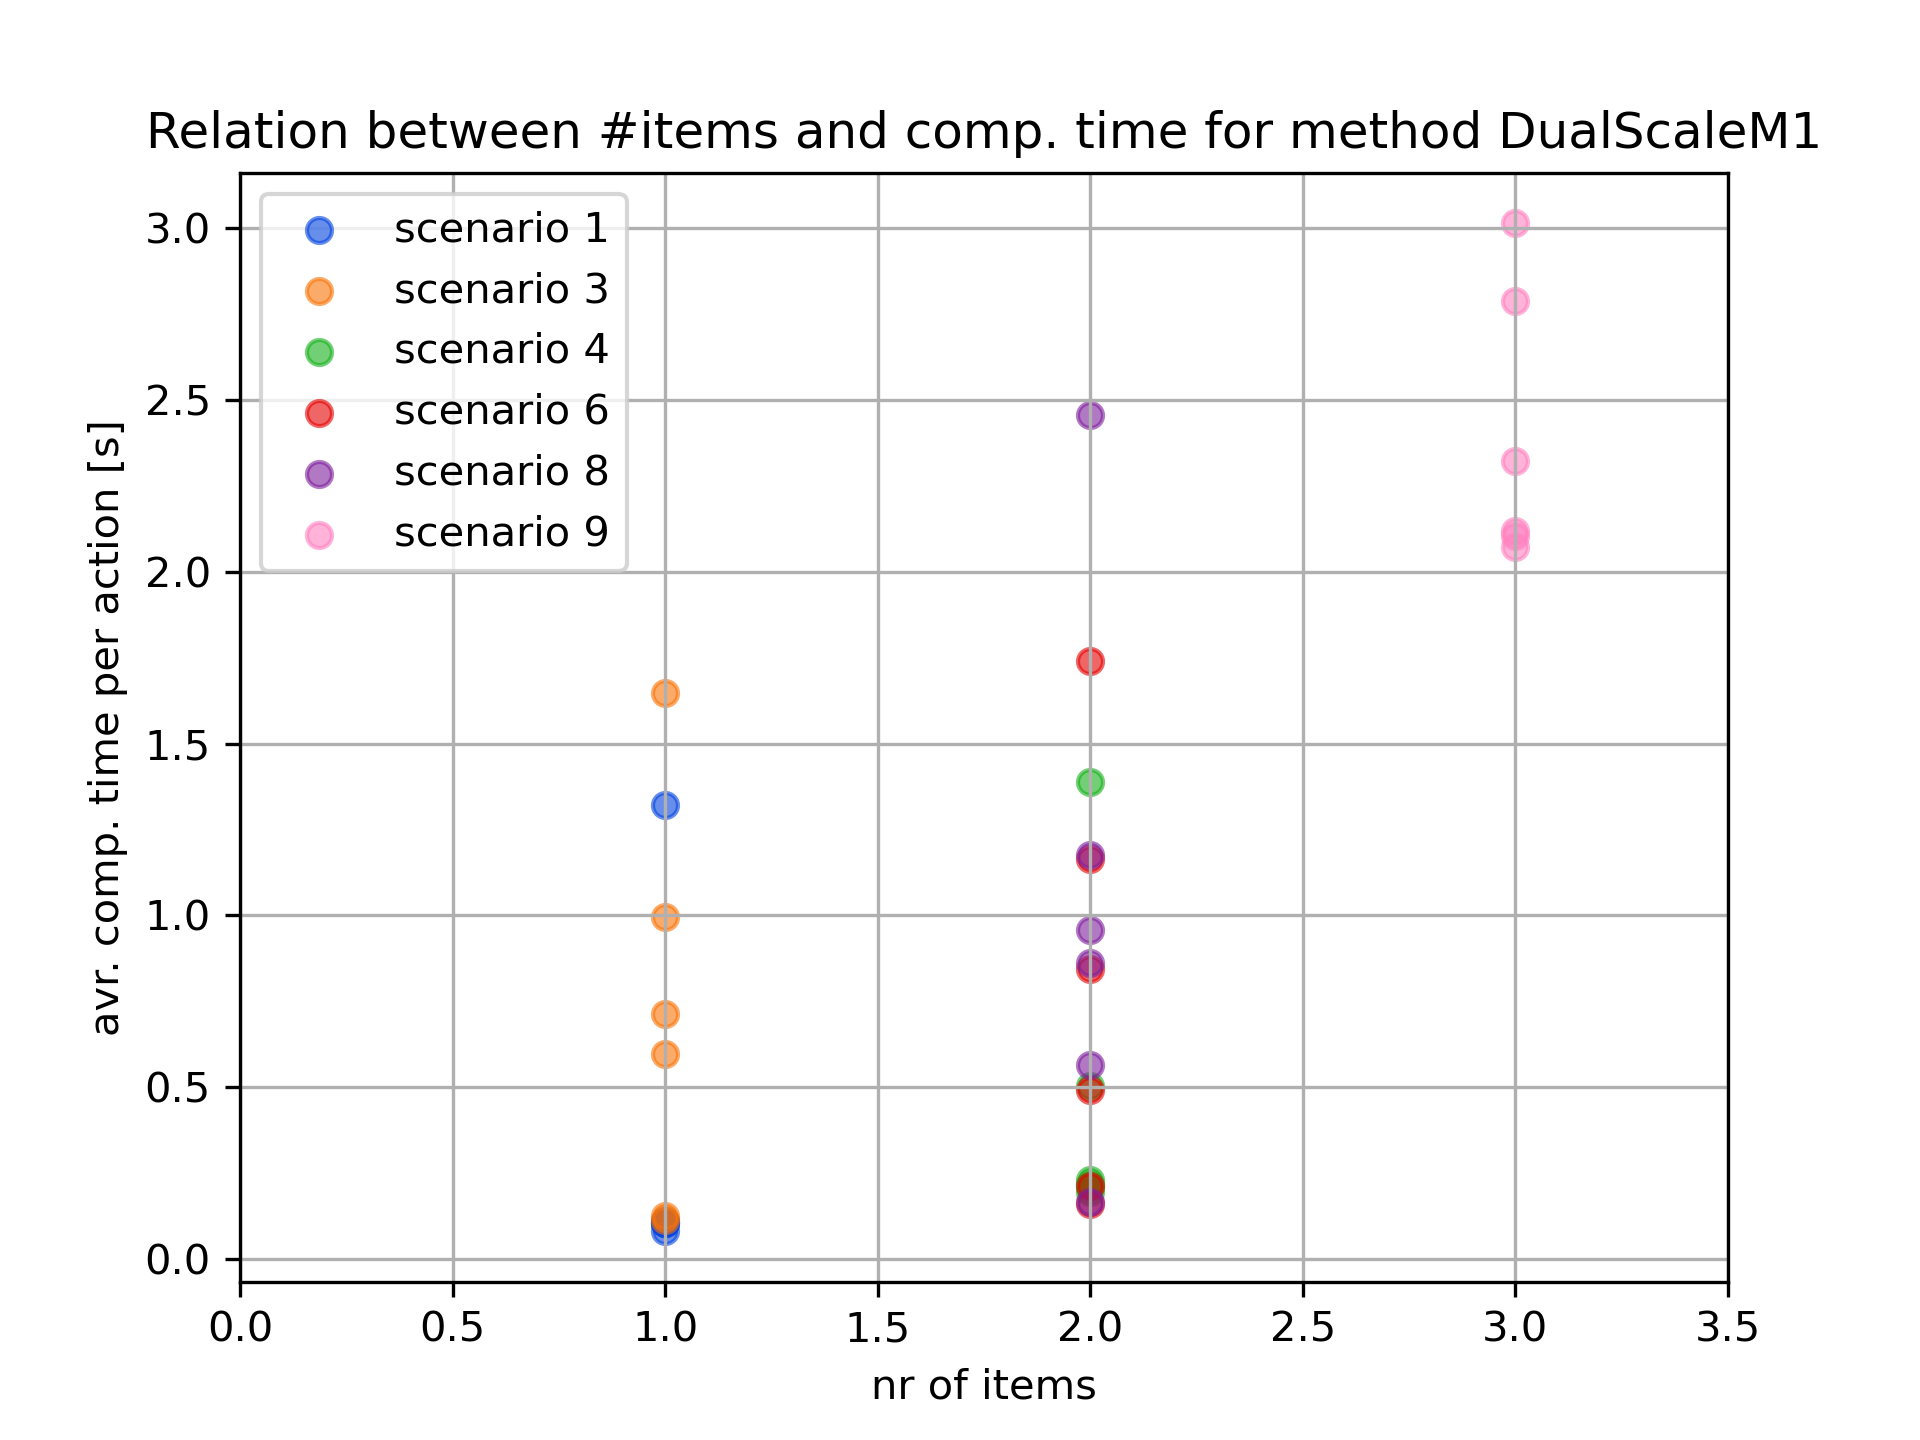
\includegraphics[width=\textwidth]{Report/images/nr_of_items/items_vs_comptime_DualScaleM1.png}
%         \caption{Caption}
%         \label{subfig:my_label}
%     \end{subfigure}
%     \hfill
%     \begin{subfigure}[b]{0.49\textwidth}
%         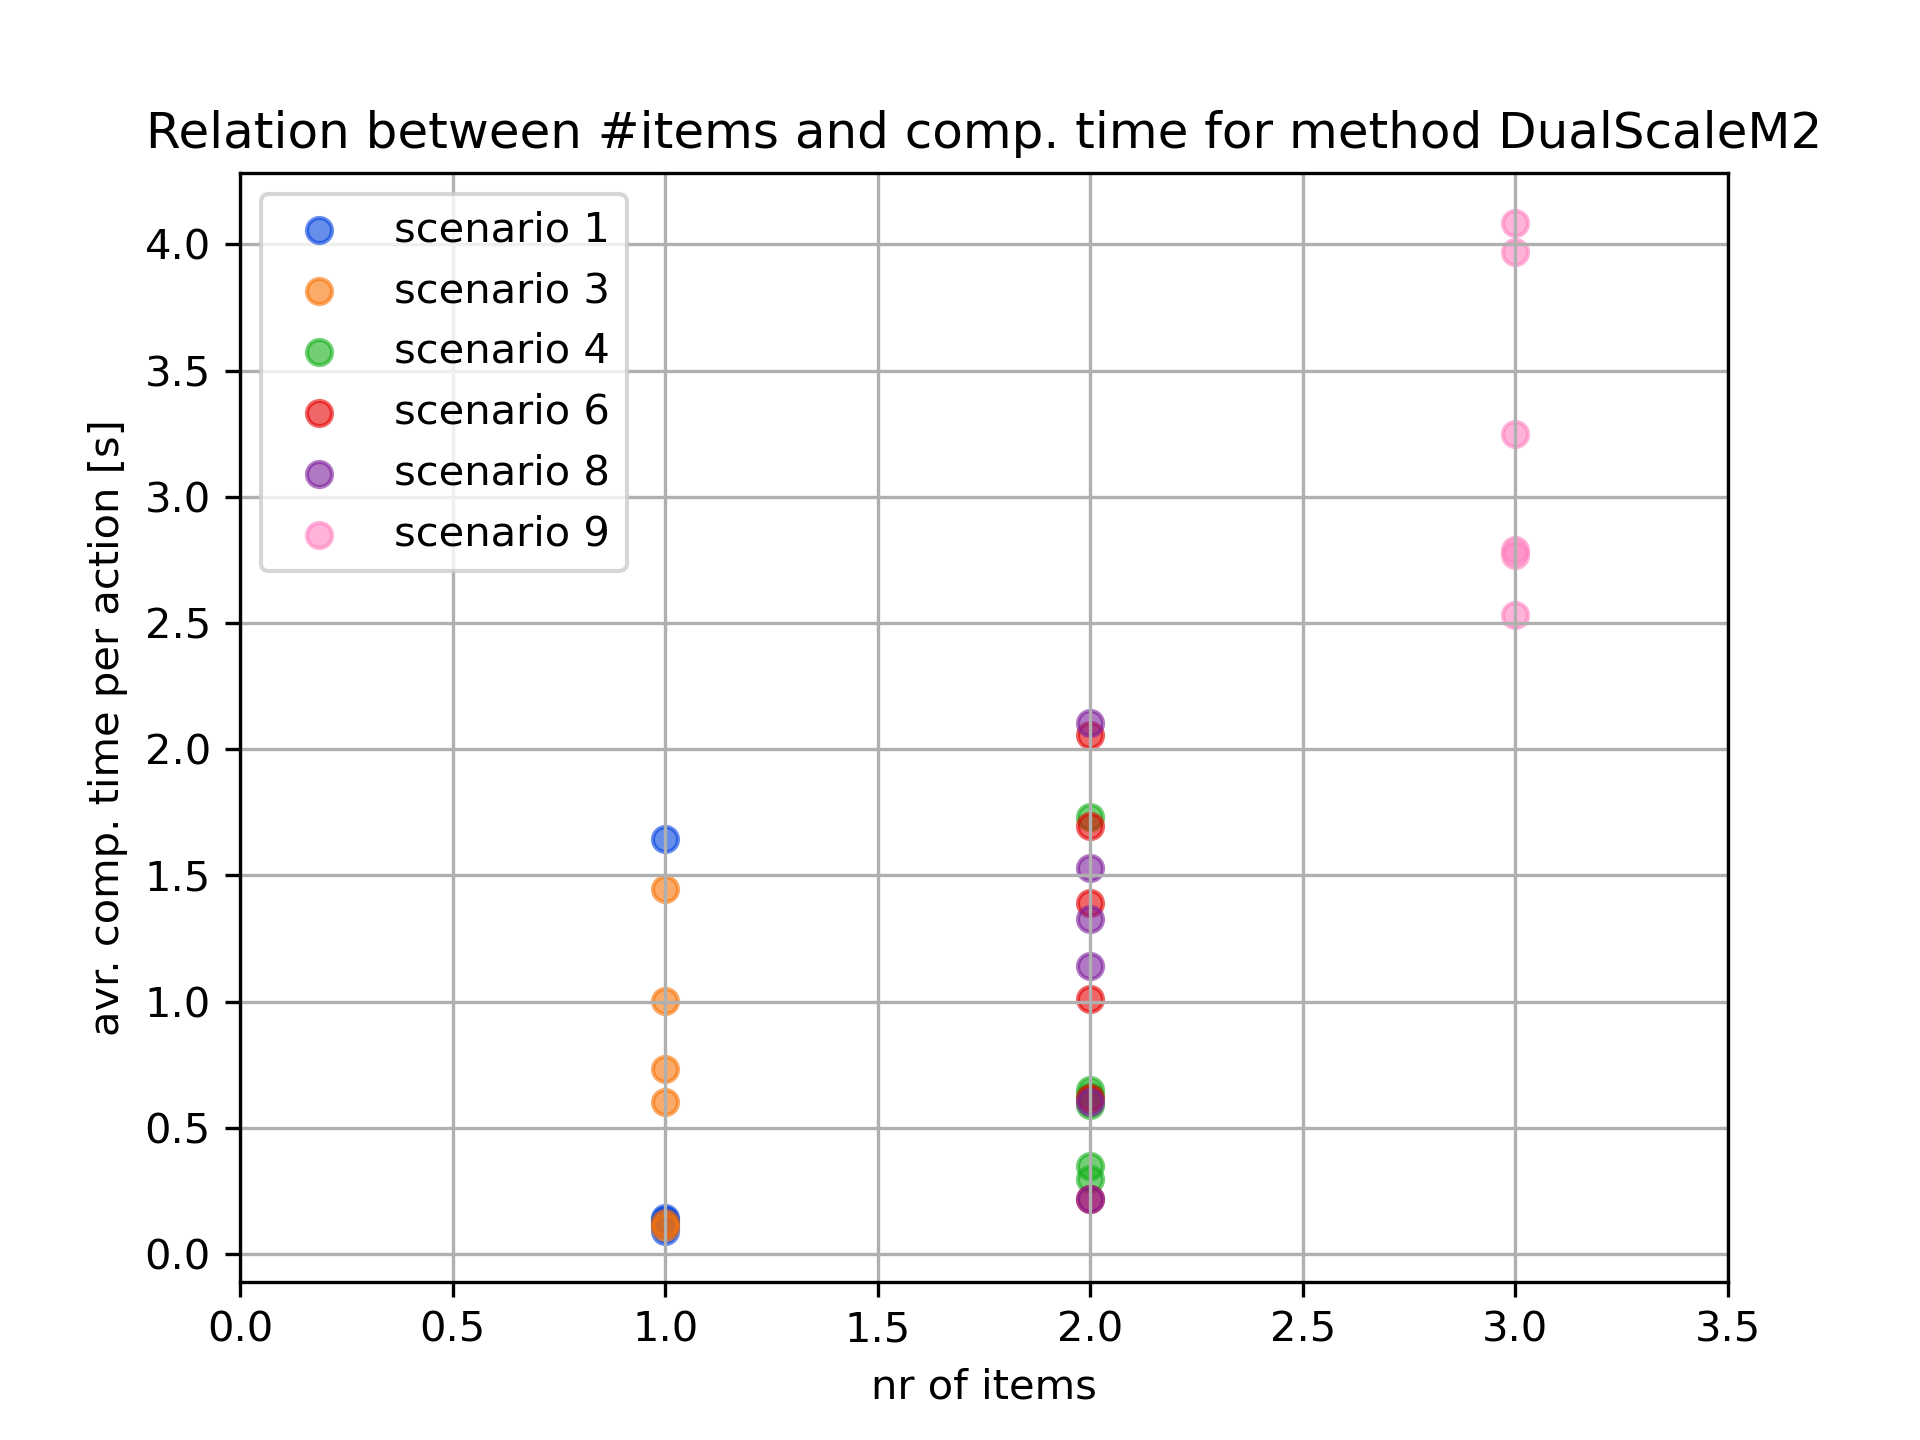
\includegraphics[width=\textwidth]{Report/images/nr_of_items/items_vs_comptime_DualScaleM2.png}
%         \caption{Caption}
%         \label{subfig:my_label}
%     \end{subfigure}
%     \hfill
%     \begin{subfigure}[b]{0.49\textwidth}
%          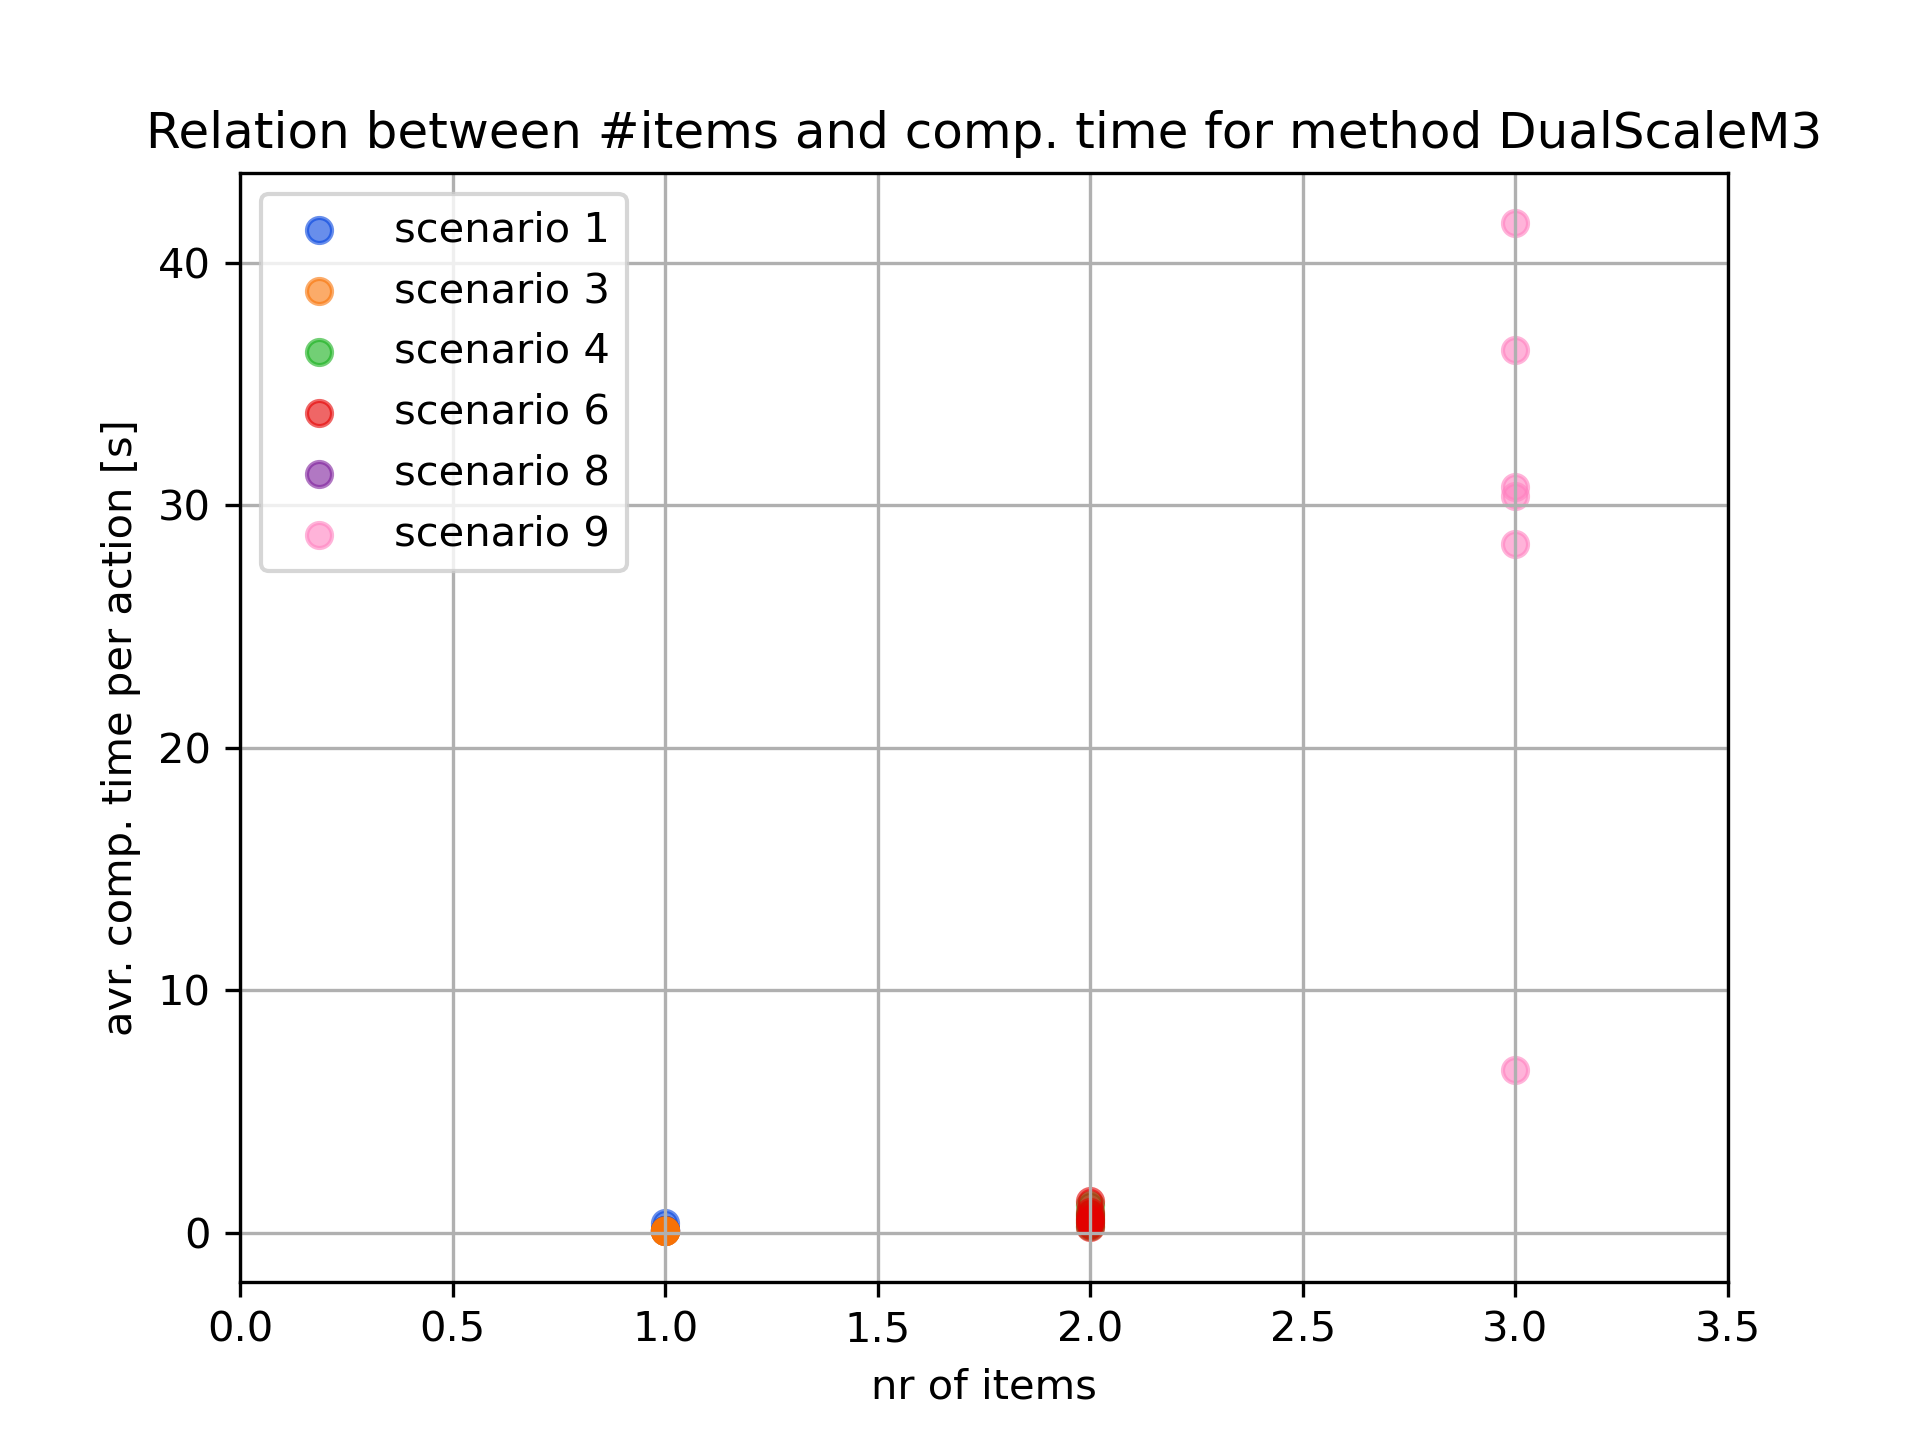
\includegraphics[width=\textwidth]{Report/images/nr_of_items/items_vs_comptime_DualScaleM3.png}
%         \caption{Caption}
%         \label{subfig:my_label}
%     \end{subfigure}
%      \caption{Blabliblub}
%     \label{fig:my_label}
% \end{figure}

%%%%%%%%%%%%%%%%%%%%%%%%%%%%%%%%%%%%%%%%%%%%%%%%%%%%%%%%%%%%%%%%%%%
%%%%%%%%%%%%%%%%%%%%%%%%%%%%%%%%%%%%%%%%%%%%%%%%%%%%%%%%%%%%%%%%%%%
\section{Corner Cases}
In this section the reasoning abilities of the three MultiScale methods are compared on two scenarios highlighting the weakness of the agents. The first problem shown in figure \ref{fig:M1_prob01} demonstrates that Method 02 and Method 03 have better lower layer reasoning than Method 01. In (\subref{subfig:problem1_M1}) and (\subref{subfig:problem1_M2}) a snapshot of the Method 01 respectively Method 02 agent is shown. In the task the item is located right at the corner of one of multiple belief peaks, such that it was not spotted by the navigation action. For method 01 the top layer decided to go to node $n_0^{l0}$ as soon as the majority of the belief peak was observed, as the coarse discretisation of layer 0 does not reflect that some part of the belief peak is still right in front of the agent. Similarly, in the bottom most right room the search was more thorough than the one left to it. As the belief in $n_3^{l0}$ decreased under a certain threshold, layer 0 chose to go the another node. The lower layers of Method 01 execute the action of the layer above in as little time as possible and can not correct for the top layers inaccuracy. \\
The Method 02 agent has better lower layer reasoning than Method 01 and finds the item right away. As for Method 01, the top layer chooses to go to $n_0^{l0}$. The lower layers in Method 02 have access to the value function of the layer above and can choose to first explore the current states before completing the higher layer action. Layer 1 chose a \texttt{look\_around} action and observes the item, leading to a better solution than the one of Method 01. \\

\begin{figure}
    \centering
    \begin{subfigure}[b]{0.49\textwidth}
        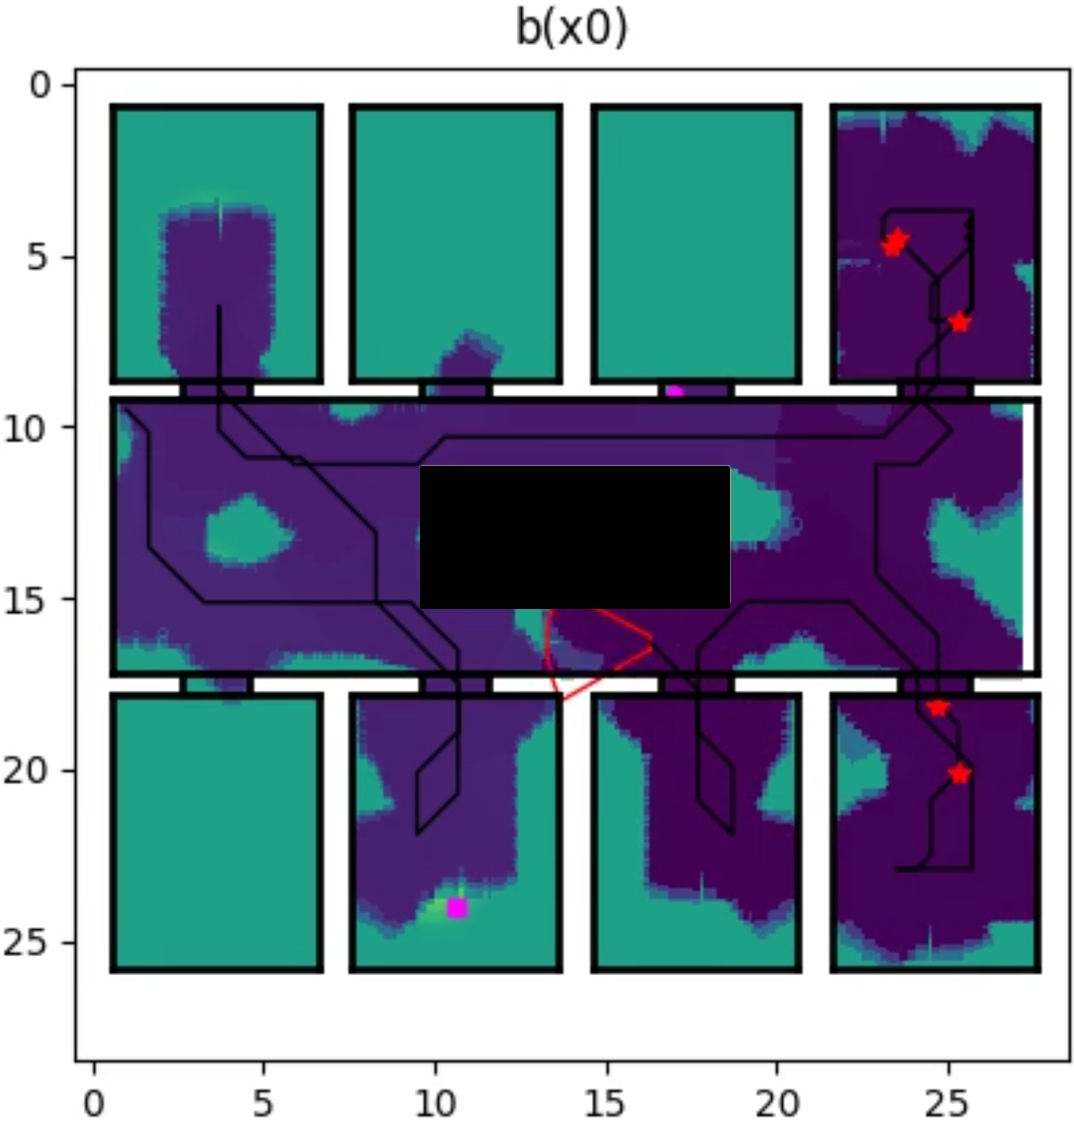
\includegraphics[width=\textwidth]{Report/images/experiments/M1_envbig_problem1_blackbox.png}
        \caption{Method 01}
        \label{subfig:problem1_M1}
    \end{subfigure}
    \begin{subfigure}[b]{0.49\textwidth}
         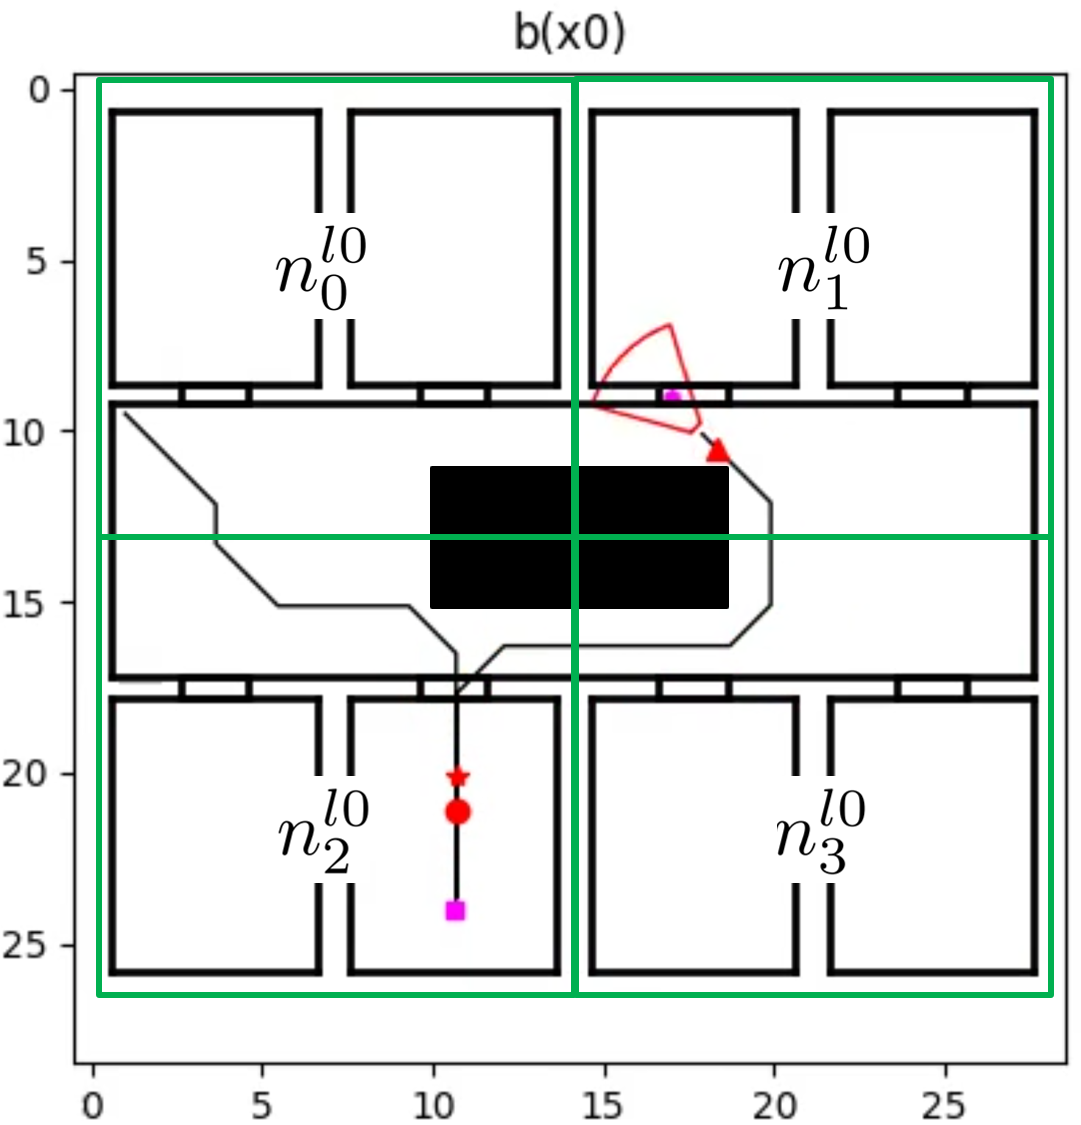
\includegraphics[width=\textwidth]{Report/images/experiments/M2_envbig_problem1_nodes.png}
        \caption{Method 02}
        \label{subfig:problem1_M2}
    \end{subfigure}
    \caption{Demonstration of inconsistent search behaviour of method 01 shown in (a) compared to method 02 in (b). The Method 01 agent missed the item right at the corner of the belief peak and continued its search in other rooms. Some rooms are searched much more thoroughly than others. Method 02 spends more time exploring the first room and finds the item right away. The black lines show the previous path of the agent, the red stars are \texttt{look\_around} action, the red circle is a pickup action and the red triangle is the \texttt{release} action.}
    \label{fig:M1_prob01}
\end{figure}

The second example shown in figure \ref{fig:M1_prob02} explores a scenario where both Method 01 (figure (\subref{subfig:problem2_M1})) and Method 02 choose a suboptimal path to get to the target location due to coarse resolution of the top layer. Method 03 (figure (\subref{subfig:problem2_M3})) can correct for the inaccuracies and chooses the shorter path. Consider the layer 0 discretisation for the large office environment in (\subref{subfig:problem2_M1}). The item shown as a pink square lies within node $n_0^{l0}$ and its goal location in $n_3^{l0}$. There is no direct connection between $n_0^{l0}$ and $n_3^{l0}$ so the layer 0 POMDP has to choose either to go over $n_1^{l0}$ or over $n_2^{l0}$ to get to $n_3^{l0}$. Due to the symmetry of the nodes layout layer 0 can not reason which path is better suited and chooses the longer path over $n_2^{l0}$. The lower layers POMDPs of both Method 01 and Method 02 execute the proposed action of the above layer. In Method 03, the lower layers have complete freedom and are only guided through the value function of the layer above. The lower layers recognize that the agent is closer to $n_1^{l0}$ than to $n_2^{l0}$ and choose the shorter way.

%%%%%%%%%%%%%%%%%%%%%%%%%%%%%%%%%%%%%%%%%%%%%%%%%%%%%%%%%%%%%%
%%%%%%%%%%%%%%%%%%%%%%%%%%%%%%%%%%%%%%%%%%%%%%%%%%%%%%%%%%%%
\begin{figure}
    \centering
    \begin{subfigure}[b]{0.49\textwidth}
        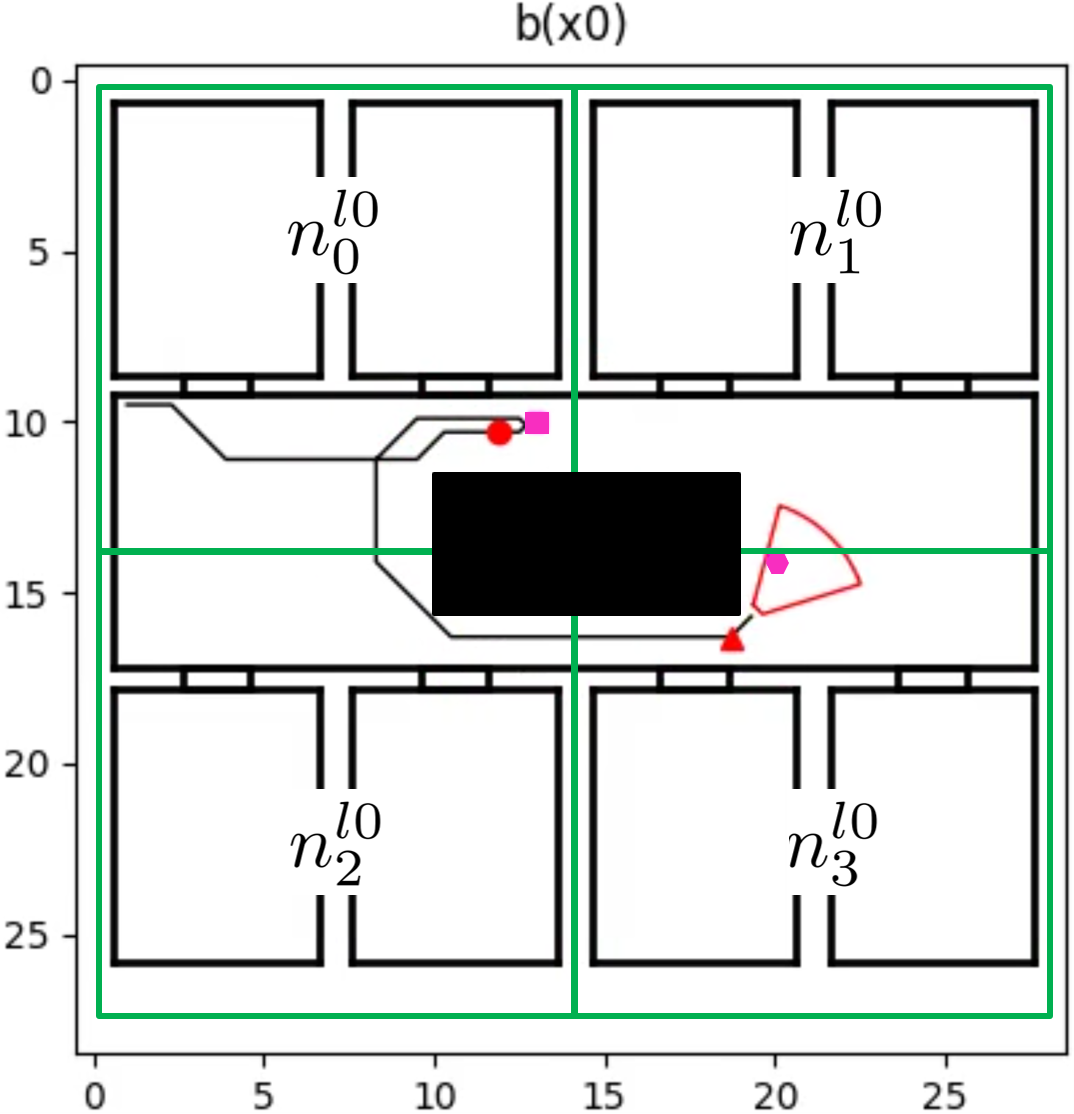
\includegraphics[width=\textwidth]{Report/images/experiments/M1_envbig_problem2_nodes.png}
        \caption{Method 01}
        \label{subfig:problem2_M1}
    \end{subfigure}
    \begin{subfigure}[b]{0.49\textwidth}
         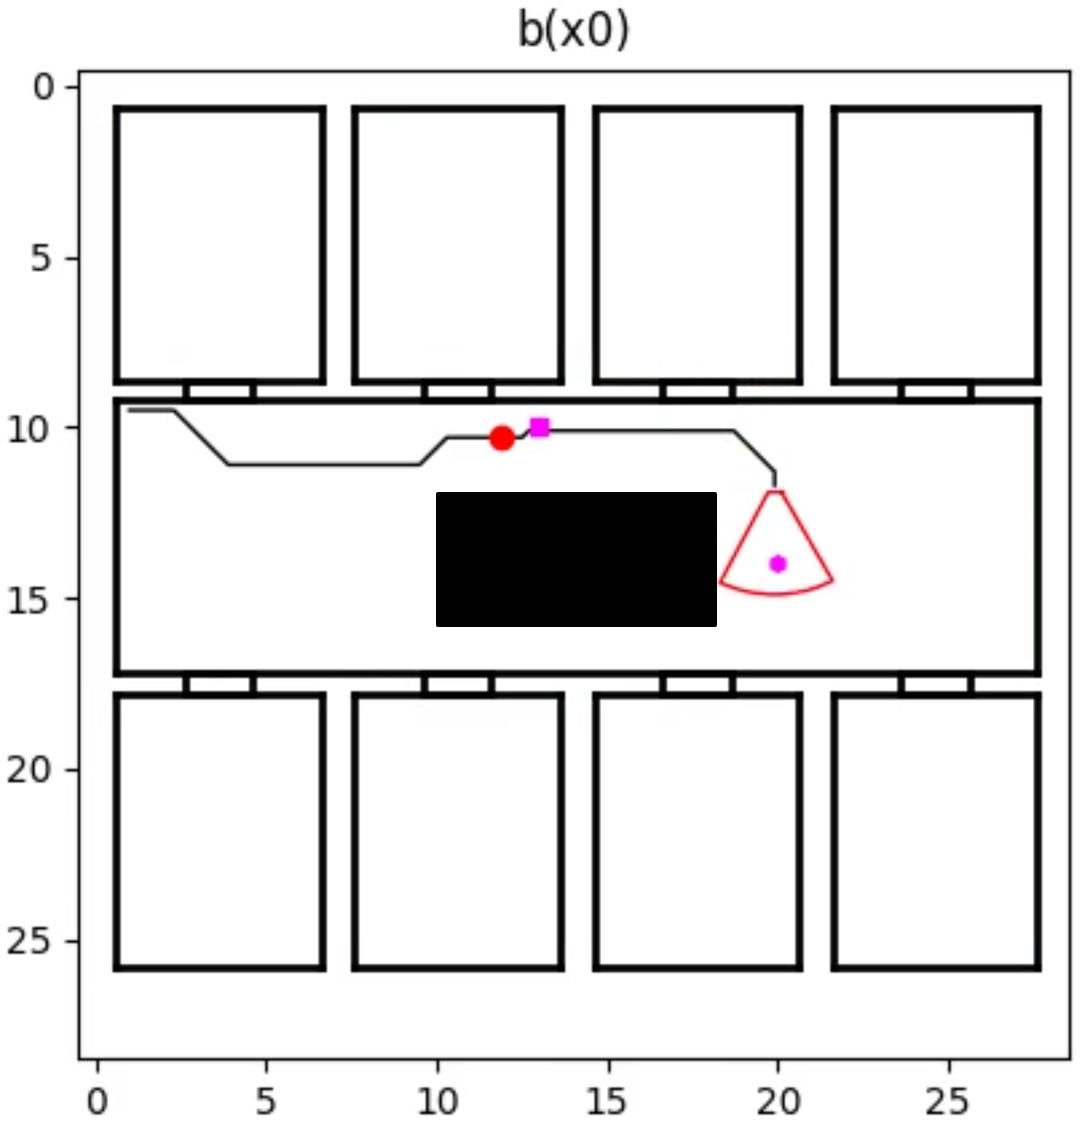
\includegraphics[width=\textwidth]{Report/images/experiments/M3_envbig_problem2_blackbox.png}
        \caption{Method 03}
        \label{subfig:problem2_M3}
    \end{subfigure}
    \caption{Demonstration of limited lower layer reasoning for method 01 shown in (a) compared to the better reasoning of method 03 in (b). Because of the coarse resolution, layer 0 is not able to correctly reason if the path over $n_1^{l1}$ or over $n_2^{l1}$ is faster for reaching the goal location. Method 03 is not restricted to follow the higher layer actions and correctly reasons that the path over $n_1^{l0}$ is faster.}
    \label{fig:M1_prob02}
\end{figure}